%%%%%%%%%%%%%%%%%%%%%%%%%%%%%%%%%%%%%%%%%%%%%%%%%%%%%%%%%%%%%%%%%%%%%%%%%%%%%%%%
%%%%%%%%%%%%%%%%%%   Vorlage für eine Abschlussarbeit   %%%%%%%%%%%%%%%%%%%%%%%%
%%%%%%%%%%%%%%%%%%%%%%%%%%%%%%%%%%%%%%%%%%%%%%%%%%%%%%%%%%%%%%%%%%%%%%%%%%%%%%%%

% Erstellt von Maximilian Nöthe, <maximilian.noethe@tu-dortmund.de>
% ausgelegt für lualatex und Biblatex mit biber

% Kompilieren mit
% lualatex dateiname.tex
% biber dateiname.bcf
% lualatex dateiname.tex
% lualatex dateiname.tex
% oder einfach mit:
% make

\documentclass[
  tucolor,
  BCOR=12mm,     % 12mm binding corrections, adjust to fit your binding
  parskip=half,  % new paragraphs start with half line vertical space
  open=any,      % chapters start on both odd and even pages
  cleardoublepage=plain,  % no header/footer on blank pages
]{tudothesis}

\renewcommand*\chapterheadstartvskip{\vspace*{-\topskip}}
\renewcommand*\chapterheadendvskip{\vspace*{1\baselineskip plus .1\baselineskip minus .167\baselineskip}}

% Warning, if another latex run is needed
\usepackage[aux]{rerunfilecheck}

% just list chapters and sections in the toc, not subsections or smaller
\setcounter{tocdepth}{1}

%------------------------------------------------------------------------------
%------------------------------ Sprache und Schrift: --------------------------
%------------------------------------------------------------------------------
\usepackage{fontspec}
\defaultfontfeatures{Ligatures=TeX}  % -- becomes en-dash etc.

% german language
\usepackage{polyglossia}
\setdefaultlanguage{german}

% for english abstract and english titles in the toc
\setotherlanguages{english}

% intelligent quotation marks, language and nesting sensitive
\usepackage[autostyle]{csquotes}

% microtypographical features, makes the text look nicer on the small scale
\usepackage{microtype}

%------------------------------------------------------------------------------
%------------------------ Für die Matheumgebung--------------------------------
%------------------------------------------------------------------------------

\usepackage{amsmath}
\usepackage{amssymb}
\usepackage{mathtools}
\usepackage{physics}

% Enable Unicode-Math and follow the ISO-Standards for typesetting math
\usepackage[
  math-style=ISO,
  bold-style=ISO,
  sans-style=italic,
  nabla=upright,
  partial=upright,
]{unicode-math}
\setmathfont{Latin Modern Math}

% nice, small fracs for the text with \sfrac{}{}
\usepackage{xfrac}


%------------------------------------------------------------------------------
%---------------------------- Numbers and Units -------------------------------
%------------------------------------------------------------------------------

\usepackage[
  locale=DE,
  separate-uncertainty=true,
  per-mode=symbol-or-fraction,
]{siunitx}
\sisetup{math-micro=\text{µ},text-micro=µ}

%------------------------------------------------------------------------------
%-------------------------------- tables  -------------------------------------
%------------------------------------------------------------------------------

\usepackage{booktabs}       % stellt \toprule, \midrule, \bottomrule

%------------------------------------------------------------------------------
%-------------------------------- graphics -------------------------------------
%------------------------------------------------------------------------------

\usepackage{graphicx}
\usepackage{grffile}

% allow figures to be placed in the running text by default:
\usepackage{scrhack}
\usepackage{float}
\floatplacement{figure}{htbp}
\floatplacement{table}{htbp}

% keep figures and tables in the section
\usepackage[section, below]{placeins}


%------------------------------------------------------------------------------
%---------------------- customize list environments ---------------------------
%------------------------------------------------------------------------------

\usepackage{enumitem}

%------------------------------------------------------------------------------
%------------------------------ Bibliographie ---------------------------------
%------------------------------------------------------------------------------

\usepackage[
  backend=biber,   % use modern biber backend
  autolang=hyphen, % load hyphenation rules for if language of bibentry is not
                   % german, has to be loaded with \setotherlanguages
                   % in the references.bib use langid={en} for english sources
]{biblatex}
\addbibresource{references.bib}  % die Bibliographie einbinden
\DefineBibliographyStrings{german}{andothers = {{et\,al\adddot}}}

%------------------------------------------------------------------------------
%------------------------------ Sonstiges: ------------------------------------
%------------------------------------------------------------------------------

\usepackage[pdfusetitle,unicode,linkbordercolor=tugreen]{hyperref}
\usepackage{bookmark}
\usepackage[shortcuts]{extdash}
\usepackage{bbm}

%------------------------------------------------------------------------------
%-------------------------    Angaben zur Arbeit   ----------------------------
%------------------------------------------------------------------------------

\author{Timo Gräßer}
\title{Der Inverse Faraday Effekt in Mott-Isolatoren}
\date{2017}
\birthplace{Lüdenscheid}
\chair{Lehrstuhl für Theoretische Physik I}
\division{Fakultät Physik}
\thesisclass{Bachelor of Science}
\submissiondate{15. August 2017}
\firstcorrector{Prof.~Dr.~Götz S. Uhrig}
\secondcorrector{Prof.~Dr.~Joachim Stolze}

% tu logo on top of the titlepage
\titlehead{
\includegraphics[height=1.5cm]{logos/tu-logo.pdf}}

\begin{document}
\frontmatter
%\thispagestyle{empty}
\setcounter{page}{2}
\section*{Hinweise}
Empfohlen wird die Verwendung dieser Vorlage mit der jeweils aktuellsten TeXLive Version (Linux, Windows) bzw. MacTeX Version (MacOS).
Aktuell ist dies TeXLive 2016. Download hier:
\begin{center}
  \ttfamily\url{https://www.tug.org/texlive/}
\end{center}
Bei Verwendung von TexLive Versionen 2014 und älter sollte
die Zeile
\begin{center}
\verb+\RequirePackage{fixltx2e}+ 
\end{center}
als erste Zeile der Präambel noch vor der Dokumentenklasse eingefügt werden.
Dies lädt diverse Bugfixes für LaTeX, die ab TexLive 2015 Standard sind.

Die Vorlage \texttt{thesis.tex} ist für die Kompilierung mit \texttt{lualatex} ausgelegt, mit wenigen Anpassungen kann sie aber auch mit \texttt{pdflatex} oder \texttt{xelatex} verwendet werden. 
Die Dokumentenklasse \texttt{tudothesis.cls} kann mit allen drei Programmen verwednet werden.

Achten Sie auch auf die Kodierung der Quelldateien.
Bei Verwendung von Xe\LaTeX\ oder Lua\LaTeX\ (empfohlen) müssen die
Quelldateien UTF-8 kodiert sein.
Bei Verwendung von pdf\LaTeX\ nutzen Sie die Pakete \texttt{inputenc} und \texttt{fontenc} mit der korrekten Wahl der Kodierungen.

Eine aktuelle Version dieser Vorlage steht unter 
\begin{center}
  \ttfamily\url{https://github.com/maxnoe/tudothesis}
\end{center}
zur Verfügung.

Alle verwendeten Pakete werden im \LaTeX{} Kurs von Pep et al.\ erklärt:
\begin{center}
  \ttfamily\url{http://toolbox.pep-dortmund.org/notes}
\end{center}

Für Rückmeldungen und bei Problemen mit der Klasse oder Vorlage, bitte ein \emph{Issue} auf GitHub aufmachen oder eine Email an
\href{mailto:maximilian.noethe@tu-dortmund.de}{maximilian.noethe@tu-dortmund.de} schreiben.

Wenn Sie die Dokumentenklasse mit der Option \texttt{tucolor} laden, werden verschiedene Elemente in TU-Grün gesetzt.

\maketitle

% Gutachterseite
\makecorrectorpage

% hier beginnt der Vorspann, nummeriert in römischen Zahlen
\thispagestyle{plain}

\section*{Kurzfassung}
Hier steht eine Kurzfassung der Arbeit in deutscher Sprache inklusive der Zusammenfassung der
Ergebnisse.
Zusammen mit der englischen Zusammenfassung muss sie auf diese Seite passen.

\section*{Abstract}
\begin{english}
The abstract is a short summary of the thesis in English, together with the German summary it has to fit on this page.
\end{english}

\tableofcontents

\mainmatter
% Hier beginnt der Inhalt mit Seite 1 in arabischen Ziffern
\chapter{Einleitung}
\label{ch:einleitung}

Der inverse Faraday Effekt ist ein bedeutendes Phänomen in der Magnetooptik. Er beschreibt
die Anregung einer Magnetisierung in einem Material durch die Bestrahlung mit polarisiertem Licht
und kann somit Anwendungen in technischen Bereichen finden, wie z.B. in der Daten-Speicherung und -Übertragung.
Zudem kann der Effekt zur Erzeugung von Spinwellen genutzt werden, da diese entstehen,
wenn die Magnetisierung in einem magnetisch geordneten Material aus dem Gleichgewicht gebracht wird.
In einem Experiment mit dem Titel "Magnon Accumulation by Clocked Laser Excitation as Source of
Long-Range Spin Waves in Transparent Magnetic Films"\cite{jäckl} wurden beispielsweise ferri-magnetische
Eisen-Granat-Proben mit Laserpulsen angeregt, um kohärente Spinwellen zu generieren.
Dabei diente zirkular polarisiertes Laserlicht mittels des inversen Faraday Effekts als externe periodische Kraft auf
die magnetischen Momente der Proben.
Die Verwendung von ferri-magnetischen Eisen-Granaten ist auf ihre isolierende und somit transparente Eigenschaft
zurückzuführen.  \cite{hertel, jäckl}

Im Rahmen dieser theoretischen Bachelorarbeit wird der inverse Faraday Effekt in einem Mott-Isolator modelliert und analysiert, um
Erkenntnisse für die Erzeugung einer Magnetisierung durch polarisiertes Licht, beispielsweise in Bezug auf Spinwellen-Experimente, zu erhalten.
Dazu werden zunächst theoretische Grundlagen und Konventionen zum Verständnis der physikalischen und mathematischen Inhalte
der Arbeit in Kapitel \ref{ch:theorie} dargelegt. Im darauffolgenden Kapitel \ref{ch:isolatormodelle} werden verschiedene theoretische
Isolatoren und Isolator-Modelle vorgestellt, wobei der Schwerpunkt auf dem Mott-Isolator liegt.
Kapitel \ref{ch:ife} umfasst eine kurze Herleitung zur angeregten Magnetisierung durch den inversen Faraday Effekt in Metallen und Isolatoren.
Die Modellierungen und Ergebnisse dieser Arbeit werden in Kapitel \ref{ch:ergebnisse} präsentiert. Hierbei wird mehrfach die Eignung der Modellierung
des Mott-Isolators anhand der theoretischen Erwartungen aus den Kapiteln \ref{ch:theorie} und \ref{ch:isolatormodelle} überprüft.
Darüber hinaus wird die Abhängigkeit der angeregten Magnetisierung im Mott-Isolator von der Frequenz und der Amplitude des
polarisierten Lichts analysiert.

\chapter{Theoretische Grundlagen und Konventionen}

Vektoren fett
Im Folgenden wird in natürlichen Einheiten gerechnet, das heißt unter anderem
\begin{align}
  \hbar = 1.
\end{align}
ortsraum

\section{Die Schrödingergleichung}
\label{sec:schroedingergleichung}

Die zeitliche Entwicklung eines quantenmechanischen, nicht-relativistischen Zustandes $\ket{\Psi}$ ist durch die Schrödingergleichung
\begin{align}
  \symup{i} \frac{\partial}{\partial t} \ket{\Psi(\symbf{x},t)} = H(\symbf{x},t) \ket{\Psi(\symbf{x},t)}
  \label{eqn:schroedingergleichung}
\end{align}
gegeben. Dabei ist
\begin{align}
  H(\symbf{x},t) = -\frac1{2 m} \symbf{\nabla}^2 + V(\symbf{x},t)
  \label{eqn:hamiltonian}
\end{align}
der Hamiltonoperator mit einem beliebigen Potential $V(\symbf{x},t)$.
Wenn das Potential $V$ und somit auch der Hamiltonian $H$ zeitunabhängig ist, werden in der Schrödingergleichung \eqref{eqn:schroedingergleichung} Ort $\symbf{x}$ und Zeit $t$ mit dem Ansatz
\begin{align}
  \Psi(\symbf{x},t) = \Phi(\symbf{x})f(t)
  \label{eqn:separation}
\end{align}
separiert. Die daraus resultierende stationäre Schrödingergleichung
\begin{align}
  H \ket{\Phi(\symbf{x})} = E \ket{\Phi(\symbf{x})}
  \label{eqn:statschroedinger}
\end{align}
ist nur noch vom Ort $\symbf{x}$ abhängig und die Wellenfunktionen $\Psi(\symbf{x},t)$, die die Schrödingergleichung \eqref{eqn:schroedingergleichung} lösen, sind Eigenzustände des Hamiltonoperators $H$ zu den Eigenwerten $E$.
Wenn das Potential $V$ und der Hamiltonoperator $H$ zeitabhängig sind, kann die Schrödingergleichung \eqref{eqn:schroedingergleichung} nicht separiert werden, sondern in den meisten Fällen nur numerisch, zum Beispiel durch ein Integrationsverfahren, gelöst werden.
Nähere Informationen zur Herleitung und zur Lösung der Schrödingergleichung können \cite{schwabl} entnommen werden.

\section{Quantenmechanische Operatoren und die zweite Quantisierung}

In der Quantenmechanik sind den Observablen der klassischen Physik Operatoren zugeordnet.
Dieses Postulat wird als Korrespondenzprinzip bezeichnet.
\cite{schwabl}

Die zweite Quantisierung ist eine Darstellung von Operatoren, die sich vor allem für die Betrachtung von fermionischen Vielteilchensystemen eignet.
Grundlage für diese Darstellung sind die auf dem Fockraum definierten fermionischen Erzeugungs- und Vernichtungsoperatoren $c^\dag$ und $c$.
Diese ändern die Teilchenzahl eines fermionischen Vielteilchenzustands gemäß
\begin{align}
  c_i^{\phantom{\dag}} \ket{N_1, N_2, ..., N_i, ...} & = \pm n_i \ket{N_1, N_2, ..., N_i-1, ...} \label{eqn:vernichter}\\
  c_i^\dag \ket{N_1, N_2, ..., N_i, ...} & = \pm (1-N_i) \ket{N_1, N_2, ..., N_i+1, ...} \label{eqn:erzeuger}
\end{align}
um $1$. Dabei ist $N_i$ die Besetzungszahl des i-ten Zustands, die aufgrund des Pauliprinzips nur die Werte $0$ und $1$ annehmen kann.
Das Vorzeichen in \eqref{eqn:vernichter} und \eqref{eqn:erzeuger} entsteht durch die Antisymmetrie des Zustands. \cite{cy}

Im Folgenden werden Operatoren und Zustände ausschließlich in Ortsdarstellung angegeben und verwendet.

\section{Der Besetzungszahloperator}

Alle fermionischen Vielteilchenzustände sind Eigenfunktionen der Besetzungszahloperatoren
\begin{align}
  n_i = c_i^\dag c_i^{\phantom{\dag}},
  \label{eqn:besetzer}
\end{align}
wobei die zugehörigen Eigenwerte jeweils die Besetzungszahlen $n_i$ der i-ten Zustände sind.
Der Wertebereich der Eigenwerte ist daher ebenfalls auf $0$ und $1$ beschränkt.
\cite{cy}

\section{Der Spinoperator}

Die Indizes der Erzeugungs- und Vernichtungsoperatoren werden im Folgenden um einen zusätzlichen Parameter $\sigma$, der die Spinausrichtung eines Elektrons angibt, erweitert.
Die Ein-Teilchen-Zustände des fermionischen Vielteilchensystems spalten sich dadurch jeweils in zwei im Ort entartete Zustände auf, die sich nur in der Spin-Magnetquantenzahl $\sigma$ unterscheiden.
Der Parameter $\sigma$ kann die Werte $\sigma = \frac12$, für Spin Up ($\uparrow$), und $\sigma = -\frac12$, für Spin Down ($\downarrow$), annehmen.

Um den Gesamtspin $S$ eines fermionischen Vielteilchensystems zu ermitteln, wird zunächst der vektorartige Spinoperator für das Einteilchensystem
\begin{align}
  S & = \begin{pmatrix*}[r]
    S_x \\
    S_y \\
    S_z
  \end{pmatrix*}
  \label{eqn:spinoperator}
\end{align}
eingeführt. Die Quantisierungsachse wird im Folgenden in z-Richtung gelegt, sodass die Einteilchenzustände Eigenfunktionen des $S_z$-Operators zu den Eigenwerten $\sigma$ sind.
Der $S_x$- und der $S_y$-Operator werden dann mit
\begin{align}
  S_x & = \frac12 \left(S_+ + S_- \right) & S_y &= \frac1{2i} \left(S_+ - S_- \right)
  \label{eqn:leiteroperatorenausdruck}
\end{align}
durch die Spin-Leiteroperatoren $S_+$ und $S_-$ ausgedrückt. Die Wirkung der Spin-Leiteroperatoren auf einen fermionischen Einteilchenzustand mit Spin Up oder Spin Down ist durch
\begin{align}
  S_+ \ket{\uparrow} & = 0 & S_+ \ket{\downarrow} & = \ket{\uparrow} \label{eqn:spluswirkung}\\
  S_- \ket{\uparrow} & = \ket{\downarrow} & S_- \ket{\downarrow} & = 0 \label{eqn:sminuswirkung}
\end{align}
gegeben. Das Anwenden des $S_+$-Operators auf einen Einteilchenzustand entspicht dem Vernichten eines Elektrons mit Spin Down gefolgt vom Erzeugen
eines Elektrons mit Spin Up. Dies gilt auch für den $S_-$-Operator mit vertauschten Spins. Daraus folgt Darstellung der Spin-Leiteroperatoren in zweiter Quantisierung
\begin{align}
  S_+ & = c_\uparrow^\dag c_\downarrow^{\phantom{\dag}} & S_- & = c_\downarrow^\dag c_\uparrow^{\phantom{\dag}}. \label{eqn:leitersecondquant}
\end{align}
Die Eigenwertgleichungen für den $S_z$-Operator
\begin{align}
  S_z \ket{\uparrow} &= \frac12 \ket{\uparrow} & S_z \ket{\downarrow} &= -\frac12 \ket{\downarrow}
\end{align}
führen auf die Darstellung des Operators in zweiter Quantisierung
\begin{align}
  S_z = \frac12 (n_\uparrow -  n_\downarrow) = \frac12 (c_\uparrow^\dag c_\uparrow^{\phantom{\dag}} - c_\downarrow^\dag c_\downarrow^{\phantom{\dag}}) \label{eqn:szsecondquant}.
\end{align}
\cite{schwabl}

Aus den Gleichungen \eqref{eqn:spinoperator} und \eqref{eqn:leiteroperatorenausdruck} folgt der $S^2$-Operator für ein fermionisches Einteilchensystem
\begin{align}
  S^2 & = S_z^2 + \frac12 \left( S_+ S_- + S_- S_+ \right)
  \label{eqn:squadoperatorein}
\end{align}
Durch summieren der Einteilchenoperatoren $S_{+,i}$, $S_{-,i}$ und $S_{z,i}$ über alle Zustandsniveaus $i$ folgt aus den Gleichungen \eqref{eqn:squadoperatorein} die Darstellung des $S^2$-Operators in zweiter Quantisierung für ein fermionisches Vielteilchensystem
\begin{align}
  S^2 & = \frac14 \left(\sum_{i} n_{\uparrow,i} - n_{\downarrow,i}\right)^2 +
  \frac12 \left( \sum_{i,j} c_{\uparrow,i}^\dag c_{\downarrow,i}^{\phantom{\dag}} \cdot c_{\downarrow,j}^\dag c_{\uparrow,j}^{\phantom{\dag}} + c_{\downarrow,i}^\dag c_{\uparrow,i}^{\phantom{\dag}} \cdot c_{\uparrow,j}^\dag c_{\downarrow,j}^{\phantom{\dag}} \right).
  \label{eqn:squadoperatorviel}
\end{align}
Die Vielteilchenzustände sind Eigenfunktionen des $S^2$-Operators zu den Eigenwerten $S(S+1)$.
\cite{???}

\chapter{Isolator-Modelle}
\label{ch:isolatormodelle}

In diesem Kapitel werden verschiedene Arten von theoretischen Isolatoren aufgezählt und mehrere Isolator-Modelle vorgestellt.
Die Modelle werden dabei auf Nächst-Nachbar-Wechselwirkungen und eindimensionale Gittersysteme mit periodischen Randbedingungen reduziert.
Festkörper können anhand ihrer elektrischen Leitfähigkeit in Metalle und Isolatoren unterteilt werden,
wobei der physikalische Unterschied in der Bandstruktur der Elektronendispersion liegt.
In Metallen ist das Leitungsband bei beliebigen Temperaturen teilweise gefüllt, sodass die Elektronen theoretisch mit beliebig kleinen Energien angeregt werden können.
Daher ist der Realteil der Leitfähigkeit endlich und es kann ein Stromfluss generiert werden.
Bei Isolatoren befindet sich die Fermienergie $\epsilon_F$ in einer Bandlücke der Bandstruktur, sodass das unterste Leitungsband am Temperaturnullpunkt unbesetzt ist.
Der Realteil der Leitfähigkeit von Isolatoren ist somit gering, da für die Anregung eines Elektrons mindestens die Energie der Bandlücke aufgebracht werden muss,
und verschwindet für $T \to 0$. Im folgenden Abschnitt werden verschiedene Ursachen für die Enstehung eines leeren Leitungsbandes aufgezählt und damit
theoretische Isolatoren klassifiziert. \cite{czycholl,gebhard}

\section{Klassifizierung von Isolatoren}
\label{sec:klassifizierung}

Ein Metall-Isolator-Übergang kann durch mehrere Phänomene, die den Elektronentransport im Festkörper beeinflussen, auftreten.
In diesem Abschnitt werden verschiedene theoretische Isolatoren vorgestellt, die ihre Isolator-Eigenschaft jeweils durch eines dieser Phänomene erhalten.
Bei einem Band-Isolator verursacht die direkte Wechselwirkung zwischen den Elektronen und dem periodischen Gitterpotential eine Bandlücke und ein leeres Leitungsband.
Dabei muss die Anzahl an Elektronen pro Elementarzelle gerade sein, da nur in diesem Fall ein leeres Leitungsband entstehen kann.
Der Peierls-Isolator erhält seine Isolator-Eigenschaft durch den Einfluss eines effektiven Gitterpotentials, welches aus der Bildung von statischen Gitterverzerrungen
und damit verbundenen Ladungsdichtewellen durch die Wechselwirkung zwischen Elektronen und Gitter entsteht.
Beim Anderson-Isolator liegt die Ursache für die geringe Leitfähigkeit in der Wechselwirkung zwischen Elektronen und Gitterfehlern.
Die Unordnung im Gittersystem, die durch die Gitterfehler hervorgerufen wird, führt zu einer Lokalisierung der Elektronen und somit zu einem Metall-Isolator-Übergang.
Der Mott-Isolator ist durch eine nicht vernachlässigbare Coulomb-Wechselwirkung der Elektronen untereinander charakterisiert.
Dabei wird zwischen dem Mott-Hubbard-Isolator, bei welchem die Isolator-Eigenschaft aus der Ladungskorrelation resultiert,
und dem Mott-Heisenberg-Isolator, bei welchem die Spinkorrelation für die Isolator-Eigenschaft ausschlaggebend ist, unterschieden.
Im folgenden Abschnitt wird ein grundlegendes Festkörper-Modell vorgestellt, das zur Beschreibung der aufgezählten Isolatoren jeweils unterschiedlich erweitert werden kann.
\cite{czycholl,gebhard}

\section{Das Tight-Binding-Modell}

Um Aussagen über Bandstrukturen von Festkörpern zu machen, werden verschiedene Ansätze für das Verhalten der Elektronen im Gitterpotential gemacht.
Während die Elektronen im Bloch-Theorem als quasifrei in einem schwachen periodischen Gitterpotential angenommen werden, so werden sie
im Tight-Binding-Modell als gebunden und an den diskreten Gitterplätzen lokalisiert angenommen. Das Tight-Binding-Modell ist unter anderem Grundlage für das Hubbard-Modell,
das zur Beschreibung von Hubbard-Mott-Isolatoren dient, und wird deshalb im Folgenden kurz beschrieben.

Mit der Annahme einer starken Bindung fallen die Wellenfunktionen der Elektronen eines isolierten Atoms signifikant mit mit dem Abstand zum Kern ab.
Wenn der Abstand zwischen den Atomen eines Festkörpers hinreichend groß ist, überlappen sich die Wellenfunktionen der Elektronen eines Atoms näherungsweise nicht mit
den Coulomb-Potentialen der umgebenden Atome. Somit sind die Eigenzustände und -energien des atomaren Problems auch Eigenzustände und -energien des gesamten Festkörpersystems.
Die Dynamik ist dann durch diskrete Sprünge der Elektronen zwischen den Gitterplätzen, hervorgerufen durch den Tunneleffekt, gegeben.
Ausgehend von diesen Annahmen, lautet der Hamiltonoperator des Tight-Binding-Modells in zweiter Quantisierung
\begin{align}
  H_\text{Tb} = -J \sum_{i,\sigma} (c_{i+1,\sigma}^{\dag}c_{i,\sigma}^{\phantom{\dag}} + c_{i,\sigma}^{\dag}c_{i+1,\sigma}^{\phantom{\dag}}).
  \label{eqn:hamiltontb}
\end{align}
Summiert wird über alle Gitterplätze $i$ und Spinausrichtungen $\sigma \in \{ \uparrow,\downarrow \}$ der Elektronen.
Der Koeffizient $J$ gibt die Stärke der Tight-Binding-Wechselwirkung an und ist daher mit der Tunnelwahrscheinlichkeit eines Elektrons zwischen zwei Gitterplätzen korreliert. \cite{czycholl}

\section{Das Hubbard-Modell und der Hubbard-Mott-Isolator}
\label{sec:hubbardmodell}

In diesem Abschnitt wird zunächst das Zustandekommen des Metall-Mott-Hubbard-Isolator-Übergangs für ein eindimensionales Gittersystem erklärt und anschließend
eine mathematische Beschreibung des Hubbard-Modells angegeben.
Der Tight-Binding-Ansatz liefert für ein eindimensionales Gittersystem mit der Gitterkonstante $a$ die Dispersionsrelation
\begin{align}
  E(k) = -2J \cos \left(ka \right).
  \label{eqn:dispersion}
\end{align}
Diese beschreibt genau ein Energieband mit der zur Tight-Binding-Stärke korrelierten Bandbreite $W = 4J$.
Um die starke Elektron-Elektron-Wechselwirkung, die im Mott-Isolator angenommen wird, zu realisieren, wird der Hubbard-Parameter $U$, welcher die Energiedifferenz
zwischen einem doppelt besetzten Gitterplatz $(\uparrow \downarrow;0)$ und zwei einzeln besetzten Gitterplätzen $(\uparrow; \downarrow)$ angibt, eingeführt.
Es kann gezeigt werden, dass sich das Energieband \eqref{eqn:dispersion} für einen endlichen Hubbard-Parameter $U$ in zwei Energiebänder aufspaltet. Diese überlappen
für $U \ll W$ und driften für einen ansteigenden Hubbard-Parameter $U$ auseinander.
Etwa bei $U=W$ entsteht eine Lücke für Ladungsanregungen, sodass ein Metall-Mott-Hubbard-Isolator-Übergang stattfindet.

Um den Hamiltonoperator des Hubbard-Modells aufzustellen, wird der Hamiltonoperator des Tight-Binding-Modells wie in der vorgestellten Herleitung um einen
Potentialterm, der abhängig von $U$ ist, erweitert. Da der Potentialterm genau dann von Null verschieden ist, wenn eine Doppelbesetzung $n_{i,\uparrow} n_{i,\downarrow} = 1$ vorliegt,
ergibt sich
\begin{align}
  H_\text{Hubb} = H_\text{Tb} + U \sum_{i} n_{i,\uparrow} n_{i,\downarrow},
  \label{eqn:hamiltonhubb}
\end{align}
wobei über die Gitterplätze $i$ summiert wird.
Zu diesem Hamiltonoperator folgt mit dem Ansatz aus Abschnitt \ref{sec:stromoperator} für ein Gittersystem aus $N$ Gitterplätzen der
über alle Gitterplätze gemittelte Stromoperator
\begin{align}
  \mathcal{J} = \frac{\symup{i}J}{N} \sum_{i,\sigma} (c_{i+1,\sigma}^{\dag}c_{i,\sigma}^{\phantom{\dag}} - c_{i,\sigma}^{\dag}c_{i+1,\sigma}^{\phantom{\dag}}).
  \label{eqn:stromoperator}
\end{align}
\cite{czycholl,gebhard,uhrig}

\section{Das Heisenberg-Austausch-Modell und der Heisenberg-Mott-Isolator}

In diesem Abschnitt wird zunächst der Übergang des Mott-Hubbard-Isolators in den Mott-Heisenberg-Isolator erklärt
und anschließend das Heisenberg-Austausch-Modell, welches zur Beschreibung eines Mott-Heisenberg-Isolators dient, beschrieben.
Für einen Hubbard-Parameter $U \gg J$ ist jeder Gitterplatz des halbgefüllten Mott-Hubbard-Isolators
im Grundzustand einfach besetzt, da dies energetisch am günstigsten ist.
Die gesamte Dynamik des Systems ist dann durch eine Spin-Austausch-Wechselwirkung der Elektronen gegeben und
der Mott-Hubbard-Isolator geht in den Mott-Heisenberg-Isolator über.

Im Mott-Heisenberg-Isolator können zwei Elektronen benachbarter Gitterplätze ihre Spinausrichtungen, wenn diese antiparallel zueinander stehen, in virtuellen Prozessen austauschen.
Der Tight-Binding-Term im Hamiltonoperator des Hubbard-Modells \eqref{eqn:hamiltonhubb} wird
als Störung behandelt. Für die virtuellen Austausch-Prozesse zwischen zwei benachbarten Elektronen mit antiparalleler Spinausrichtung ergeben sich
in zweiter Ordnung Störungstheorie die Energiedifferenzen
\begin{align}
  \Delta E_{\uparrow \downarrow} = - \frac{2J^2}{U}.
  \label{eqn:Ediffantipar}
\end{align}
Ein Sprung zwischen zwei benachbarten Elektronen mit paralleler Spinausrichtung ist aufgrund des Pauliprinzips nicht möglich, weshalb der Energieunterschied
\begin{align}
  \Delta E_{\uparrow \uparrow} = 0.
  \label{eqn:Ediffpar}
\end{align}
beträgt. Um den Mott-Heisenberg-Isolator mathematisch zu beschreiben, wird das Hubbard-Modell für $U \gg J$
mit dem Heisenberg-Austausch-Modell verglichen. Der zugehörige Hamiltonoperator lautet
\begin{align}
  H_\text{Spin} = t \sum_{i} (\symbf{S}_i \symbf{S}_{i+1} + C),
  \label{eqn:hamiltonspincj}
\end{align}
wobei die Summe über alle Gitterplätze läuft. Durch den Vergleich der Relationen \eqref{eqn:Ediffantipar} und \eqref{eqn:Ediffpar}
mit den Energiedifferenzen der unterschiedlichen Spinkonfigurationen im Heisenberg-Austausch-Modell
ergeben sich der Heisenberg-Parameter
\begin{align}
  t = \frac{4 J^2}{U}
  \label{eqn:spint}
\end{align}
und die Konstante $C = -\tfrac14$.
Daraus und aus der Darstellung des $\symbf{S}^2$-Operators in zweiter Quantisierung \eqref{eqn:squadoperatorviel} folgt die Darstellung des Hamiltonoperators zur Beschreibung eines
Mott-Heisenberg-Isolators in zweiter Quantisierung
\begin{align}
  \begin{split}
    H_\text{Spin} = \, \, \, & \frac{t}{4} \left(\sum_{i} \left(n_{\uparrow,i} - n_{\downarrow,i}\right)\right)^2 \\
    & + \frac{t}{2} \sum_{i} \left( c_{\uparrow,i}^\dag c_{\downarrow,i}^{\phantom{\dag}} \cdot c_{\downarrow,i+1}^\dag c_{\uparrow,i+1}^{\phantom{\dag}} +
    c_{\downarrow,i}^\dag c_{\uparrow,i}^{\phantom{\dag}} \cdot c_{\uparrow,i+1}^\dag c_{\downarrow,i+1}^{\phantom{\dag}} - \frac12 \right).
  \end{split}
  \label{eqn:hamiltonspin2}
\end{align}
\cite{gebhard,uhrig}

\chapter{Der inverse Faraday Effekt}
\label{ch:ife}

In diesem Kapitel wird der inverse Faraday Effekt in Metallen und Isolatoren behandelt.
Der inverse Faraday-Effekt (im Folgenden mit IFE abgekürzt) beschreibt die Anregung eines Kreisstroms in einem Material durch das Bestrahlen mit zirkular polarisiertem Licht.
Der angeregte Kreisstrom induziert dabei eine Magnetisierung, die gegebenenfalls mit geordneten magnetischen Momenten im Material wechselwirkt.
In den folgenden Abschnitten wird ein Ausdruck für diese durch den IFE angeregte Magnetisierung in Metallen und Isolatoren hergeleitet.
Dabei werden der Magnetfeld-Anteil und die räumliche Oszillation des zirkular polarisierten Lichts vernachlässigt und
quantenmechanische Effekte der Elektronen im Festkörper ignoriert. \cite{hertel} \cite{jäckl}

\section{Der inverse Faraday Effekt in Metallen}

Die Grundannahme für die Herleitung des IFE in Metallen ist, dass sich die Elektronen wie ein wechselwirkungsfreies Plasma mit der
Dichte $n(\vec{x},t)$ und der Geschwindigkeit $\vec{v}(\vec{x},t)$ verhalten. Für die elektrische Stromdichte gilt
\begin{align}
  \vec{j} = n(\vec{x},t) \cdot \vec{v}(\vec{x},t) = \sigma \cdot \delta \vec{E}(\vec{x},t),
\end{align}
wobei $\sigma$ die elektrische Leitfähigkeit des Plasmas ist und
\begin{align}
  \delta \vec{E}(t) = \vec{E}_0 \symup{e}^{-\symup{i}\omega t}
\end{align}
das zeitlich oszillierende elektrische Feld des polarisierten Lichts mit der Amplitude $\vec{E}_0$ und der Kreisfrequenz $\omega$.
Ausgehend von der Kontinuitätsgleichung
\begin{align}
  \frac{\partial n(\vec{x},t)}{\partial t} + \nabla \left[n(\vec{x},t) \cdot \vec{v}(\vec{x},t)\right] = 0
\end{align}
wird durch Separation der Zeitskalen die Magnetisierung
\begin{align}
  \vec{M} = -\frac{\symup{i}}{4 \langle n \rangle \omega} \left( \sigma^* \vec{E}_0^* \times \sigma \vec{E}_0 \right)
  \label{eqn:magnetisierung}
\end{align}
hergeleitet, wobei $\langle n \rangle$ der zeitliche Mittelwert der Ladungsdichte ist. Durch Einsetzen der elektrischen
Leitfähigkeit für das Elektronenplasma
\begin{align}
  \sigma = \frac{i \langle n \rangle}{\omega}
\end{align}
folgt die im Metall induzierte Magnetisierung durch rechts- bzw. linkszirkular polarisiertes Licht, welches sich in z-Richtung ausbreitet,
\begin{align}
  \vec{M}_\text{Metall} = \pm \frac{\langle n \rangle}{4 \omega^3} \left| \vec{E}_0 \right|^2 \vec{e}_z.
  \label{eqn:metmag}
\end{align}
Nach dieser Gleichung können die magnetischen Momente in beispielsweise ferro- oder ferri-magnetischen Metallen präzise
mit einem zirkular polarisierten Laser angeregt und unter bestimmten Umständen sogar permanent manipuliert werden. \cite{hertel}

\section{Der inverse Faraday Effekt in Isolatoren}
\label{sec:ifeiso}

Bei der Herleitung des IFE in Metallen ist die einzige materialspezifische Größe, welche eingesetzt wird,
die Leitfähigkeit des Elektronenplasmas. Um eine Abschätzung für die Abhängigkeiten des IFE in einem Mott-Isolator zu generieren,
wird die elektrische Leitfähigkeit eines Isolators\cite{fließbach}
\begin{align}
  \sigma = \symup{i} \omega \mathcal{C}
\end{align}
in die Magnetisierung \eqref{eqn:magnetisierung} eingesetzt, wobei $\mathcal{C}$ eine Konstante ist, die von den Dielektrizitäts-Eigenschaften des Materials abhängt.
Daraus ergibt sich die induzierte Magnetisierung durch rechts- bzw. linkszirkular polarisiertes Licht, welches sich in z-Richtung ausbreitet,
\begin{align}
  \vec{M}_\text{Ioslator} = \pm \frac{\omega \mathcal{C}^2}{4 \langle n \rangle} \left| \vec{E}_0 \right|^2 \vec{e}_z.
  \label{eqn:isomag}
\end{align}

Aus diesem Kapitel tritt hervor, dass durch den IFE sowohl in einem Metall, als auch in einem Isolator eine endliche Magnetisierung angeregt werden kann.
Für ferrimagnetische Isolatoren ist dies auch experimentell bestätigt und zur Erzeugung von Spinwellen ausgenutzt worden\cite{jäckl}.
Mit den theoretischen Grundlagen aus Kapitel \ref{ch:theorie} und den vorgestellten Isolator-Modellen aus Kapitel \ref{ch:isolatormodelle}
wird im folgenden Kapitel \ref{ch:ergebnisse} ein Mott-Hubbard-Isolator modelliert und untersucht.
Daraufhin wird zur Untersuchung des IFE in diesem Isolator ein rotierendes E-Feld zur Modellierung von zirkular polarisiertem Licht eingeschaltet und
der Erwartungswert für den angeregten Kreisstrom berechnet. Dieser wird in Abhängigkeit von der Amplitude und der Frequenz des E-Felds aufgetragen
und mit der vorausgesagten induzierten Magnetisierung \eqref{eqn:isomag} verglichen. \cite{hertel}

\chapter{Modellierungen und Ergebnisse}
\label{ch:ergebnisse}

Die Modellierungen und Ergebnisse dieser Arbeit stützen sich auf die vorgestellten theoretischen Inhalte und werden in den folgenden Abschnitten dargelegt.
Im ersten Teil werden die in Kapitel \ref{ch:isolatormodelle} behandelten Modelle auf ein mikroskopisches, zweidimensionales, quadratisches Festkörpersystem, bestehend aus vier Gitterplätzen, angewandt.
Da jeder Gitterplatz zwei direkte Nachbarn besitzt, kann das Festkörpersystem für ortsunabhängige Betrachtungen auch als eindimensionale Kette mit periodischen Randbedingungen interpretiert werden.
Im zweiten Teil dieses Kapitels wird der in Kapitel \ref{ch:ife} vorgestellte IFE in einem Mott-Hubbard-Isolator untersucht.

Die Darstellung von Vielteilchenzuständen in erster Quantisierung aus Gleichung \eqref{eqn:vtdarstellung1quant} wird im Folgenden mit
\begin{align}
  \ket{\Psi} = \ket{k_1,...,k_{N_e}}
  \label{eqn:vtdarstellung1quantkurz}
\end{align}
abgekürzt. Bei allen Summierungen über Gitterplätze sind periodische Randbedingungen vorausgesetzt.
Numerische Diagonalisierungen von Matrizen werden mit der Funktion \textit{eig} von \textit{GNU Octave} durchgeführt.
Zum Lösen von Differentialgleichungen werden die Integrationsverfahren Runge-Kutta-5 und Runge-Kutta-8 der Funktion \textit{complex\_ode} von \textit{scipy.integrate} verwendet.
Die Werte der verwendeten Naturkonstanten $\symup{e}, \hbar, c$ und $\epsilon_0$ werden dem Lehrbuch \cite{kittel} entnommen.

\section{Analyse eines Festkörpersystems im Tight-Binding-Modell}
\label{sec:untersuchungtb}

In diesem Abschnitt wird die Dynamik eines Festkörpersystems, bestehend aus vier Niveaus, die jeweils einen Gitterplatz repräsentieren, und einem bzw. zwei Elektronen (im Folgenden abgekürzt mit 4N1E bzw. 4N2E),
im Tight-Binding-Modell analysiert. Das 4N1E-System ist in Abbildung \ref{fig:vierniveausystem} mit beispielhafter Besetzung skizziert.
\begin{figure}
  \centering
  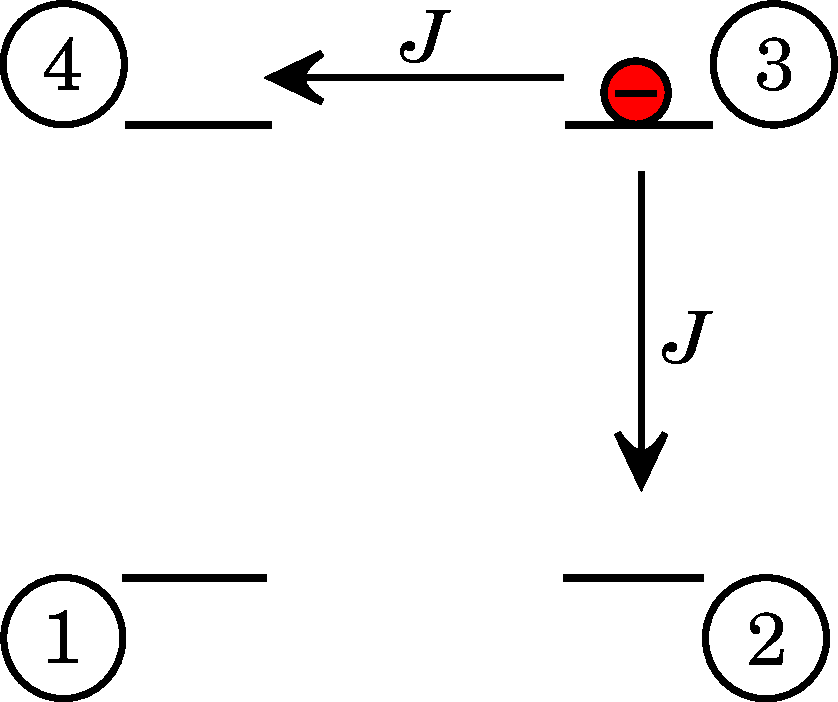
\includegraphics[height = 3.2cm]{Graphiken/vier_niveau_system.pdf}
  \caption{Skizze des 4N1E-Systems mit beispielhafter Besetzung $\ket{3}$. Die waagerechten Striche stellen die Niveaus dar, die eingekreisten Zahlen die Nummer des Gitterplatzes, der rot gefärbte Kreis das Elektron
  und die Pfeile die möglichen Sprünge des Elektrons aus der dargestellten Besetzung in Abhängigkeit von $J$.}
  \label{fig:vierniveausystem}
\end{figure}
Das eine Elektron kann in Abhängigkeit von der Tight-Binding-Stärke $J$ waagerecht oder senkrecht zwischen den Gitterplätzen springen.
Der Hilbertraum des 4N1E-Systems setzt sich aus vier Basis-Zuständen, bei denen sich das Elektron jeweils auf einem der vier Gitterplätze befindet, zusammen und ist daher vierdimensional.
Um die Dynamik zu analysieren werden zuerst die Basis-Zustände aufgestellt, daraus die vierdimensionale Hamilton-Matrix bestimmt und mit Hilfe dieser die Schrödingergleichung \eqref{eqn:schroedingergleichung} gelöst.

Zur Darstellung der Basis-Zustände wird die Konvention
\begin{align}
  \ket{i} = \ket{f_i(x)}
  \label{eqn:4N1Ezustandsvorschrift}
\end{align}
verwendet. Dabei gibt die Funktion $f_i(x)$ die Nummer des Gitterplatzes an, auf dem sich das Elektron $x$ befindet.
Der Hamiltonoperator des Systems ist in Gleichung \eqref{eqn:hamiltontb} in zweiter Quantisierung angegeben.
In Tabelle \ref{tab:4N1Ezust} sind die Basis-Zustände und in Gleichung \eqref{eqn:4N1Ehamiltonmatrix} die Matrixdarstellung des Hamiltonoperators $H$, die sich aus Gleichung \eqref{eqn:matrixelemente} ergibt, dargestellt.
Damit wird die stationäre Schrödingergleichung \eqref{eqn:statschroedinger} aufgestellt und durch Diagonalisieren der Hamilton-Matrix analytisch gelöst.
Die berechneten Energie-Eigenwerte $E_q/J$ und die Koeffizienten $\alpha_{i,q}$ der generierten Eigenzustände $\Psi_q$ sind in Tabelle \ref{tab:4N1Eeig} aufgelistet.
Die Eigenzustände ergeben sich aus der Linearkombination
\begin{align}
  \Psi_q = \sum_i \alpha_{i,q} \ket{i}.
  \label{eqn:linkomb}
\end{align}
Da das Betragsquadrat der Koeffizienten $\alpha_{i,q}$ jeweils der Besetzungswahrscheinlichkeit $P_i \in [0,1]$ für den i-ten Basis-Zustand des Systems im Eigenzustand $\Psi_q$ entspricht,
ist an die Linearkombination \eqref{eqn:linkomb} die Normierungsbedingung
\begin{align}
  \sum_i \lvert \alpha_{i,q} \rvert^2 = 1.
  \label{eqn:tbnb}
\end{align}
geknüpft.
\begin{table}[h]
  \centering
  \caption{Analytisch berechnete Eigenwerte $E_q/J$ und zugehörige Koeffizienten $\alpha_{i,q}/0.5$ der Eigenzustände $\Psi_q$ des 4N1E-Systems.}
  \begin{tabular}{S[table-format=1.0] S[table-format=2.0] S[table-format=1.0] S[table-format=1.0] S[table-format=1.0] S[table-format=2.0]}
    \toprule
    {$q$} & {$E_q/J$} & {$\alpha_{1,q}/0.5$} & {$\alpha_{2,q}/0.5$} & {$\alpha_{3,q}/0.5$} & {$\alpha_{4,q}/0.5$}\\
    \midrule
    0 & -2 & 1          & 1          & 1                  & 1                  \\
    1 & 0  & $\sqrt{2}$ & 0          & \text{$-\sqrt{2}$} & 0                  \\
    2 & 0  & 0          & $\sqrt{2}$ & 0                  & \text{$-\sqrt{2}$} \\
    3 & 2  & 1          & -1         & 1                  & -1                 \\
    \bottomrule
  \end{tabular}
  \label{tab:4N1Eeig}
\end{table}
Die Erwartung ist dadurch bestätigt, dass die Eigenenergien $E_q$ in der für das Tight-Binding-Modell vorausgesagten Bandbreite $W = 4J$ der Dispersionsrelation \eqref{eqn:dispersion} liegen.

%Die einzige Quantenzahl, in denen sich die Basis-Zustände des 4N1E-Systems unterscheiden, ist die Nummer $i$ des Gitterplatzes, an welchem das Elektron positioniert ist.
%Da alle Gitterplätze jeweils zwei direkte Nachbarn besitzen, die sich bis auf die Nummer $i$ nicht unterscheiden,
%ist die Besetzungswahrscheinlichkeit des Elektrons in den Eigenzuständen, die sich aus nicht-entarteten Eigen-Energien ergeben, gleichmäßig auf alle vier Basis-Zustände bzw. Niveaus aufgeteilt.
%Aus der Normierungsbedingung \eqref{eqn:tnbn} folgt daher für diese Eigenzustände des Systems
%\begin{align}
%  P_{i,k} = \lvert \alpha_{i,k} \rvert^2 = 0.25.
%  \label{eqn:BesetzungRot}
%\end{align}
%Das ist für die berechneten Eigenzustände $v_0$ und $v_3$ der Fall. Für die Eigenzustände zu entarteten Energie-Eigenwerten, hier $v_1$ und $v_2$ zur Energie $E_1 = E_2 = 0$, können mehrere verschiedene
%Basen gewählt werden, sodass Gleichung \eqref{eqn:BesetzungRot} nicht zwangsläufig gilt. Der physikalische Grund dafür ist, dass das Elektron bei hinreichender Energie einen Zustand,
%der sich aus einer Linearkombination der beiden Eigenzustände $v_1$ und $v_2$ ergibt, besetzt.

Um den Einfluss der Pauli-Wechselwirkung zu untersuchen, werden im nächsten Schritt die Eigenenergien eines 4N2E-Systems bestimmt.
In diesem System sind die waagerechten und senkrechten Sprünge der Elektronen zwichen den Gitterplätzen durch das Pauliprinzip eingeschränkt,
da die Doppelbesetzung eines Niveaus verhindert wird. Für das 4N2E-System ergeben sich insgesamt
\begin{align*}
  \binom{d_{\text{1e}}}{N_e} = \binom42 = 6
\end{align*}
verschiedene Basis-Zustände, wobei $d_\text{1e}$ die Hilbertraum-Dimension des 4N1E-Systems und $N_e$ die Anzahl an Elektronen ist.
Die Eigenenergien setzen sich jeweils additiv aus zwei, aufgrund des Pauliprinzips unterschiedlichen, Eigenenergien des 4N1E-Systems zusammen.
In Tabelle \ref{tab:4N2Eeigenwerte} sind die addierten Eigenenergien für das 4N2E-System aufgelistet. Auch diese liegen in der in Abschnitt \ref{sec:hubbardmodell}
vorrausgesagten Bandbreite $W = 4J$.

\begin{table}[h]
  \centering
  \caption{Additiv aus den Eigenenergien $E_q$ des 4N1E-Systems in Tabelle \ref{tab:4N1Eeig} berechnete Eigenenergien des 4N2E-Systems in Einheiten von $J$.}
  \begin{tabular}{S[table-format=2.0] S[table-format=2.0] S[table-format=1.0] S[table-format=1.0] S[table-format=1.0] S[table-format=1.0]}
    \toprule
    {$E_0/J$} & {$E_1/J$} & {$E_2/J$} & {$E_3/J$} & {$E_4/J$} & {$E_5/J$}\\
    \midrule
    -2 & -2 & 0 & 0 & 2 & 2 \\
    \bottomrule
  \end{tabular}
  \label{tab:4N2Eeigenwerte}
\end{table}

Auf Grundlage der vorgestellten Vierniveausysteme wird im Folgenden ein Mott-Hubbard-Isolator modelliert, indem die atomaren Niveaus des
beschriebenen Gittersystems jeweils in ein Spin-Up- und ein Spin-Down-Niveau aufgespalten werden.

\section{Untersuchung eines Mott-Hubbard-Isolators}
\label{sec:untersuchunghubb}

In diesem Abschnitt wird die Dynamik eines Mott-Isolators, bestehend aus vier Gitterplätzen und acht Niveaus, im Hubbard-Modell untersucht.
Jeder Gitterplatz besitzt zwei Niveaus, die sich jeweils in der Spinausrichtung $\sigma$ unterscheiden.
Auf jeweils vier Niveaus mit äquvalenter Spinausrichtung sind zwei Elektronen verteilt, sodass das System (im Folgenden mit 8N4E abgekürzt) insgesamt halbgefüllt ist.
In Abbildung \ref{fig:hubbsystem} ist eine Skizze des Systems mit beispielhafter Elektronenbesetzung abgebildet.
Die Elektronen können unter Beachtung des Pauliprinzips waagerecht oder senkrecht zwischen den Gitterplätzen auf dem jeweiligen Spin-Niveau springen.
Das 8N4E-System besteht effektiv aus zwei gekoppelten 4N2E-Systemen mit unterschiedlicher Spinausrichtung und
beinhaltet daher $6 \cdot 6=36$ Basis-Zustände bzw. umfasst einen 36D-Hilbertraum.
Mit Hilfe der Kurzschreibweise der Vielteilchenzustände \eqref{eqn:vtdarstellung1quantkurz} werden die Basis-Zustände des Systems in erster Quantisierung in dem Schema
\begin{align}
  \ket{i} = \ket{f_i(\uparrow_1),f_i(\uparrow_2); f_i(\downarrow_1),f_i(\downarrow_2)}
  \label{eqn:8N4Ezustandsvorschrift}
\end{align}
dargestellt. Dabei ist $f_i(x_\alpha)$ eine Funktion, welche den Ort des Elektrons $x_\alpha$ im i-ten Basis-Zustand des Systems angibt.
In der Bezeichnung des Elektrons $x_\alpha$ stellt $x$ die Spinausrichtung und der Index $\alpha$ die Nummer des Elektrons dar, wobei die Elektronen eines Spinniveaus gegen den Uhrzeigersinn und beginnend beim Gitterplatz $1$ durchnummeriert werden.
Diese Konvention führt automatisch dazu, dass der zweite Eintrag einer Spinausrichtung in der Darstellung der Zustände \eqref{eqn:8N4Ezustandsvorschrift} größer als der erste ist.

\begin{figure}
  \centering
  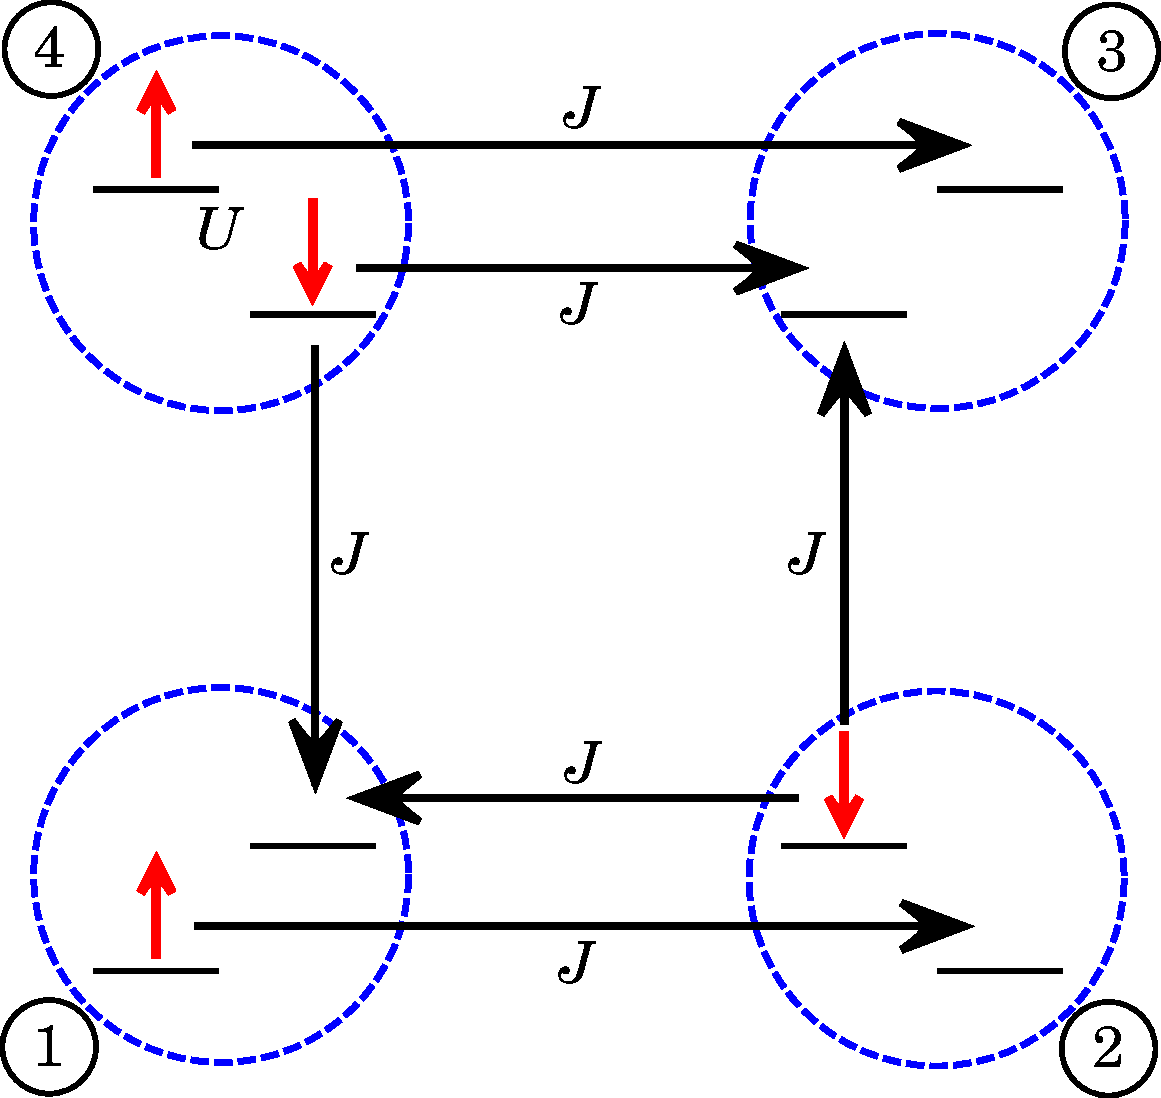
\includegraphics[height = 5.8cm]{Graphiken/hubbard_system.pdf}
  \caption{Skizze des 8N4E-Systems zur Modellierung eines Mott-Hubbard-Isolators. Die blau gestrichelten Kreise umfassen jeweils einen Gitterplatz mit zwei Niveaus
  für die jeweilige Spinausrichtung. Die roten Pfeile stellen die Elektronen inklusive ihre Spinausrichtung dar. Die Elektronen können aus der dargestellten Besetzung $\ket{1,4;2,4}$
  jeweils abhängig von $U$ und $J$ in Pfeilrichtung springen.}
  \label{fig:hubbsystem}
\end{figure}

Die Darstellungen der $36$ Basis-Zustände mit der Vorschrift \eqref{eqn:8N4Ezustandsvorschrift} sind in Tabelle \ref{tab:8N4Ehubbzust} aufgelistet.
Der Hamiltonoperator des 8N4E-Systems ist in Gleichung \eqref{eqn:hamiltonhubb} angegeben.
Um die stationäre Schrödingergleichung für das System zu lösen, wird die $36 \times 36$ - Matrix des Hamiltonoperators analog zu Abschnitt \ref{sec:untersuchungtb} aufgestellt.
Dabei bestimmt die Tight-Binding-Stärke $J$ die Nichtdiagonalelemente und der Hubbard-Parameter $U$ die Diagonalelemente der Matrix.
Diese ist in Gleichung \eqref{eqn:8N4Ehubbmatrix} angegeben.
Die vier niedrigsten Eigenenergiewerte des 8N4E-Systems sind in Tabelle \ref{tab:eigenwerte} in Einheiten von $J$ für diverse $U/J$ aufsteigend aufgelistet und in Abbildung \ref{fig:eplot} gegen $U/J$ graphisch aufgetragen.
Im Grenzfall für den Hubbard-Parameter $U/J = 0$ verschwindet die Coulomb-Wechselwirkung der Elektronen untereinander, sodass sich die 36 Eigenenergien des 8N4E-Systems additiv aus den
Eigenenergien zweier isolierter 4N2E-Systeme zusammensetzen.

\begin{figure}[H]
  \centering
  \includegraphics[height=7.4cm]{build/Hubb_eplot.pdf}
  \caption{Die vier niedrigsten Eigenenergiewerte des 8N4E-Systems in Einheiten von $J$ und in Abhängigkeit vom Hubbard-Parameter $U/J$.}
  \label{fig:eplot}
\end{figure}

Der systematische Unterschied zur Addition der Eigenenergien in Abschnitt \ref{sec:untersuchungtb} ist, dass in diesem Fall alle
Eigenenergien miteinander kombiniert werden können. Das ist darin begründet, dass sich die Elektronen des einen 4N2E-System in der Spinausrichtung $\sigma$ von
den Elektronen des anderen 4N2E-Systems unterscheiden, sodass zwischen den gekoppelten Systemen keine Pauli-Abstoßung existiert.
Aus den Kombinationen der zweifach entarteten Grundzustands-Eigenenergie eines 4N2E-Systems aus Tabelle \ref{tab:4N2Eeigenwerte} ergibt sich die vierfach entartete
Grundzustands-Eigenenergie des 8N4E-Systems $E/J = -4$ für $U/J = 0$. Da die berechneten Kurven der vier niedrigsten Eigenenergien in Abbildung \ref{fig:eplot} die Abzisse bei $E/J = -4$
schneiden, stimmen die Ergebnisse in dieser Hinsicht mit den Erwartungen überein.
Der Verlauf der Eigenenergie $E_3$ besitzt einen Knick, der durch den Differenzenquotienten zweiter Ordnung an der Stelle $U_\text{knick}/J = 2.44949$ lokalisiert wird.
Die Ursache für diesen Knick wird in Kapitel \ref{sec:spin} erklärt. Zur weiteren Überprüfung der vorgestellten Modellierung für den
Mott-Hubbard-Isolator wird im Folgenden der Übergang zum Mott-Heisenberg-Isolator untersucht und mit den Erwartungen aus Kapitel \ref{ch:isolatormodelle} verglichen.

\newpage

\section{Untersuchung eines Mott-Heisenberg-Isolators}
\label{sec:untersuchungheis}

In diesem Abschnitt wird der erwartete Übergang vom Mott-Hubbard-Isolator in den Mott-Heisenberg-Isolator für einen großen Hubbard-Parameter $U \gg J$ anhand des 8N4E-Systems überprüft.
Dafür wird die Grundzustands-Energie des 8N4E-Systems im Hubbardmodell für steigendes $U/J$ untersucht und mit der Grundzustands-Energie des 8N4E-Systems im Heisenberg-Austausch-Modell verglichen.

Die Grundzustands-Energie des 8N4E-Systems im Heisenberg-Austausch-Modell unterscheidet sich um einen konstanten Koeffizienten $-\lvert \eta \rvert$ vom Heisenberg-Parameter $t$ aus Gleichung \eqref{eqn:spint}.
Im Folgenden wird dieser Koeffizient im Hubbard-Modell näherungsweise ($\eta_\text{Hubb}$) und im Heisenberg-Austausch-Modell exakt ($\eta_\text{Spin}$) bestimmt und am Ende ein Vergleich gezogen.
Aus der Erwartung
\begin{align}
  \lim\limits_{U \to \infty} E_\text{0,hubb} = -\eta_\text{Hubb} t = -\eta_\text{Hubb} \frac{4 J^2}{U}
\end{align}
resultiert eine Geradengleichung für den Logarithmus von $E_\text{0,hubb}/J$ in Abhängigkeit vom Logarithmus von $U/J$,
\begin{align}
  \ln{\frac{\lvert E_\text{0,hubb}\rvert}{J}} = -\ln{\frac{U}{J}} + \ln{4 \eta_\text{Hubb}}.
  \label{eqn:loge0hubb}
\end{align}
Um diese zu überprüfen, ist in Abbildung \ref{fig:loglog} die numerisch berechnete logarithmische Grundzustands-Eigenenergie $E_\text{0,hubb}/J$ gegen den logarithmischen Hubbard-Parameter $U/J$ aufgetragen.
Der Verlauf von $\ln \left(\lvert E_\text{0,hubb} \rvert/J \right)$ ist für $U \to 0$ gekrümmt und geht für steigendes $U/J$ wie erwartet in eine Gerade über.
Es wird daher eine lineare Regression für $U \gg J$ durchgeführt, woraus sich durch einen Koeffizientenvergleich mit \eqref{eqn:loge0hubb} die Konstante
\begin{align}
  \eta_\text{Hubb} = 3 - \num{2e-06}
  \label{eqn:eta1}
\end{align}
ergibt. Die Durchführung und die Ergebnisse der linearen Regression sind in \ref{sec:linreg} zu finden.

In Abbildung \ref{fig:spinsystem} ist der anhand des 8N4E-Systems modellierte Mott-Heisenberg-Isolator mit beispielhafter Besetzung skizziert.
Benachbarte Elektronen mit antiparalleler Spinausrichtung können ihre Spinausrichtung in Abhängigkeit vom Heisenberg-Parameter $t$ tauschen.
Das System umfasst einen 6D-Hilbertraum und daher sechs verschiedenen Basis-Zustände. Die Basis-Zustände entsprechen den Zuständen des 8N4E-Systems aus Tabelle \ref{tab:8N4Ehubbzust}, welche vier unterschiedliche Einträge beinhalten.
Daher wird die Konvention Gleichung \eqref{eqn:8N4Ezustandsvorschrift} für dieses Modell übernommen.
\newpage
\begin{figure}[H]
  \centering
  \includegraphics[height=7.0cm]{build/Hubb_Grenz_Plot.pdf}
  \caption{Logarithmische Grundzustands-Eigenenergie $E_\text{0,hubb}/J$ in Abhängigkeit vom logarithmischen Hubbard-Parameter $U/J$ und eine Ausgleichsgerade, deren Parameter in \ref{sec:linreg} angegeben sind.}
  \label{fig:loglog}
\end{figure}

\begin{figure}[H]
  \centering
  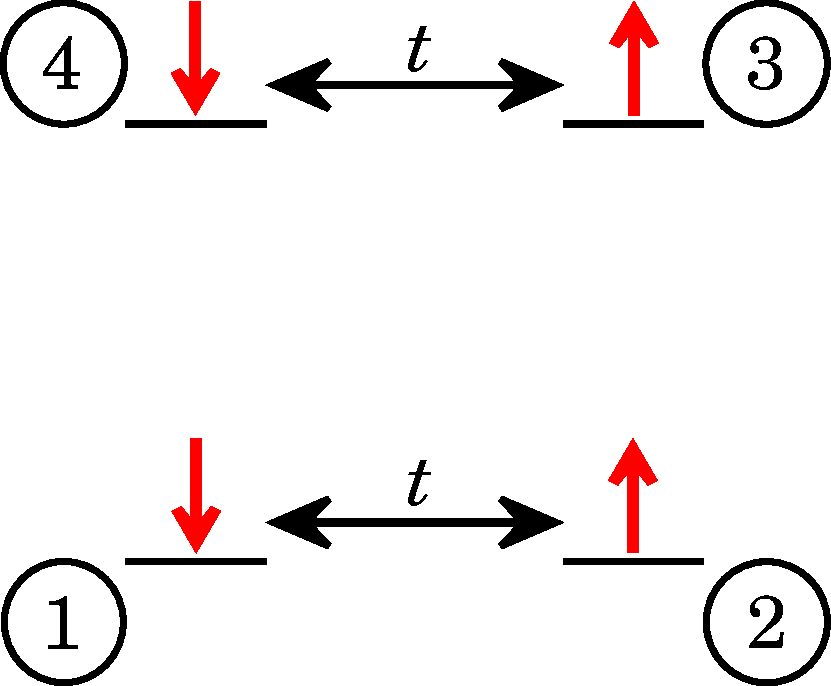
\includegraphics[height = 3.2cm]{Graphiken/heisenberg_system.pdf}
  \caption{Skizze des 8N4E-Systems zur Modellierung des Mott-Heisenberg-Isolators. Es ist nur ein Niveau pro Gitterplatz eingezeichnet, da das jeweils andere Niveau mit umgekehrter Spinausrichtung aufgrund des hohen Hubbard-Parameters $U/J$ nicht gleichzeitig besetzt wird.
  Die roten Pfeile kennzeichnen die Elektronen mit ihrer Spinausrichtung und die schwarzen Pfeile die möglichen Austausche zweier Spinausrichungen in dieser Besetzung $\ket{2,3;1,4}$ in Abhängigkeit vom Heisenberg-Parameter $t$.}
  \label{fig:spinsystem}
\end{figure}

Der Hamilton-Operator ist in Gleichung \eqref{eqn:hamiltonspin2} in zweiter Quantisierung zu finden.
In Tabelle \ref{tab:8N4Eheiszust} sind die sechs Basis-Zustände des 8N4E-Systems im Heisenberg-Austausch-Modell und in Gleichung \eqref{eqn:8N4Eheismatrix} die zugehörige $6 \times 6$ - Hamilton-Matrix dargestellt.
Die daraus berechneten Eigenenergien sind in Tabelle \ref{tab:eigenwertespin} in Einheiten von $t$ aufgelistet.

\begin{table}
  \centering
  \caption{Aus der Matrix \eqref{eqn:8N4Eheismatrix} berechnete Eigenenergiewerte des 8N4E-Systems in Einheiten von $t$.}
  \begin{tabular}{S[table-format=2.0] S[table-format=2.0] S[table-format=2.0] S[table-format=2.0] S[table-format=2.0] S[table-format=1.0]}
    \toprule
    {$E_0/t$} & {$E_1/t$} & {$E_2/t$} & {$E_3/t$} & {$E_4/t$} & {$E_5/t$}\\
    \midrule
    -3  & -2 & -1 & -1 & -1 & 0 \\
    \bottomrule
  \end{tabular}
  \label{tab:eigenwertespin}
\end{table}

Daraus wird der Wert $\eta_\text{Heis} = 3$ abgelesen. Die relative Abweichung zwischen den berechneten Koeffizienten im Hubbard-Modell und im Heisenberg-Austausch-Modell
\begin{align*}
  \Delta \eta_\text{rel} = 1 - \frac{\eta_\text{Hubb}}{\eta_\text{Heis}} = \SI{6.67e-5}{\percent}
\end{align*}
und ist gering. Durch die Ergebnisse wird der erwartete Übergang des halbgefüllten Mott-Hubbard-Isolators in den Mott-Heisenberg-Isolator für $U \gg J$
bestätigt und somit die gewählten Modellierungen erfolgreich überprüft. Bevor im letzten Abschnitt \ref{sec:untersuchungife} dieses Kapitels der IFE
im modellierten Mott-Hubbard-Isolator untersucht wird, werden die Gesamtspins der Eigenzustände ermittelt, um mögliche Energieanregungen durch den IFE im
betrachteten System zu bestimmen.

%\section{Spinanregung im Hubbard-Modell}
%
%In diesem Abschnitt wird eine Spinanregung und eine Ladungsanregung des Hubbard-Mott-Isolators für unterschiedliche Hubbard-Parameter $U/J$ untersucht,
%um Aussagen über die Energieskalen der jeweiligen Anregung zu machen. (im Folgenden abgekürzt mit $\text{8N4E}_\text{s}$), indem die Spinausrichtung eines Down-Elektrons umgedreht wird.
%Für das $\text{8N4E}_\text{s}$-System wird daher ein 4N1E-System mit einem Vierniveau-Ein-Loch-System (im Folgenden mit 4N1L abgekürzt) gekoppelt. Daraus ergibt sich ein 16D-Hilbertraum und 16 Basis-Zustände, die nach dem Schema
%\begin{align}
%  \ket{i} = \ket{f_i(\uparrow_e), f_i(\downarrow_h)}
%\end{align}
%dargestellt werden. Die Funktion $f_i(\downarrow_e)$ gibt den Ort des Spin-Down-Elektrons und die Funktion $f_i(\downarrow_h)$ den Ort des Spin-Up-Lochs im i-ten Basis-Zustand an.
%In Tabelle \ref{tab:8N4Esbasiszust} sind die Basis-Zustände in dieser Darstellung aufgelistet.
%Der Hamiltonoperator des Hubbard-Modells aus Gleichung \eqref{eqn:hamiltonhubb} wird mit Hilfe dieser Basis-Zustände als $16 \times 16$ - Matrix dargestellt.
%Dabei wird der Besetzungszahloperator $n_{i,\uparrow}$ durch $1-b_{i,\uparrow}$ ersetzt, wobei $b$ der Besetzungszahloperator für Löcher ist.
%Die Diagonalelemente der Hamiton-Matrix, die aus Basis-Zuständen resultieren, in denen Elektron $e^-$ und Loch $h^+$ am selben Ort sind, sind somit 0.
%In Tabelle \ref{tab:spinanrhammatrix} ist die Hamilton-Matrix zu sehen und in Tabelle \ref{tab:8N4Eseigenwerte} sind die analog wie in den Abschnitten \ref{sec:untersuchungtb} und \ref{sec:untersuchunghubb}
%berechneten, ersten zwei Eigenenergien in Einheiten von $J$ für verschiedene $U/J$ aufgelistet.
%
%Für $U/J = 0$ ergeben sich die Eigenenergien des $\text{8N4E}_\text{s}$-Systems durch Kombination der Eigenenergien eines 4N1E-Systemen aus Tabelle \ref{tab:4N1Eeig} und den Eigenenergien eines 4N1L-Systems.
%Mit einer Elektron-Loch-Transformation kann gezeigt werden, dass die Eigenenergien des 4N1L-Systems denen des 4N1E-Systems entsprechen.
%Die Erwartung ist daher, dass die Grundzustandsenergie des $\text{8N4E}_\text{s}$-Systems für $U/J = 0$ den Wert
%\begin{align}
%  E_0/J = -4
%\end{align}
%annimmt. Dies tritt auch aus den numerischen Rechnungen hervor (siehe Tabelle \ref{tab:8N4Eseigenwerte}).
%
%Die Grundzustandsenergie $E_0/J$ des $\text{8N4E}_\text{s}$-Systems entspricht außerdem für alle $U/J$ der Eigenenergie des ersten angeregten Zustands im 8N4E-System.
%Der Grund dafür wird in Abschnitt \ref{sec:spin} diskutiert.

\section{Ermittlung des Gesamtspins}
\label{sec:spin}

In diesem Abschnitt wird der Gesamtspin $S$ der Eigenzustände $\Psi$ des modellierten Mott-Hubbard-Isolators untersucht.
Aus den Gleichungen \eqref{eqn:squadoperatorviel} und \eqref{eqn:skommutator} folgt der Erwartungswert des $\symbf{S}^2$-Operators für einen Eigenzustand $\Psi$ des 8N4E-Systems
\begin{align}
  \bra{\Psi} \symbf{S}^2 \ket{\Psi} & = \bra{\Psi} S_- S_+ \ket{\Psi} = \left(S_+ \ket{\Psi}\right)^\dag S_+ \ket{\Psi} = S(S+1).
  \label{eqn:spin8N4E}
\end{align}
Der $S_+$-Operator ersetzt bei Anwendung auf einen Basis-Zustand des 8N4E-Systems ein Spin-Down Elektron durch ein Spin-Up Elektron. Somit bildet er den Eigenzustand $\Psi$, der auf dem 36D-Hilbertraum des 8N4E-Systems definiert ist, linear
auf einen Zustand eines in der Spinausrichtung angeregten 8N4E-Systems mit einem 16D-Hilbertraum ab. Für das angeregte 8N4E-System werden 16 Basis-Zustände nach der Vorschrift
\begin{align}
  \ket{i} = \ket{f_i(\uparrow_{h^+}),f_i(\downarrow_{e^-})}
  \label{eqn:8N4Espinvorschrift}
\end{align}
aufgestellt, wobei $h^+$ ein Loch und $e^-$ ein Elektron darstellt.
Mit Hilfe dieser Basis und der Darstellung des $S_+$-Operators in zweiter Quantisierung
\begin{align}
  S_+ = \sum_{i} c_{\uparrow,i}^\dag c_{\downarrow,i}^{\phantom{\dag}}
\end{align}
wird die Matrixdarstellung des Operators errechnet. Die Basis-Zustände sind in Tabelle \ref{tab:spluszustände} und die $16 \times 36$ - Matrix in Tabelle \eqref{eqn:splusmatrix} dargestellt.
Damit werden die Gesamtspins des 8N4E-Systems für diverse $U/J$ berechnet.
Wenn die Eigenzustände $\Psi_q$ für jedes $U/J$ nach den Werten der zugehörigen Eigenenergien geordnet sind, treten Änderungen in den Gesamtspins $S_q$ für unterschiedliche $U/J$ auf.
An der Stelle $U_\text{spin}/J = 2.44949$, die mit dem Differenzenquotienten erster Ordnung lokalisiert wird, ändert sich der Spinerwartungswert der nach den Eigenenergien geordneten Eigenvektoren $\Psi_3$, $\Psi_4$ und $\Psi_5$ gemäß
\begin{align*}
  U < U_\text{spin}/J: \quad\quad S_3=0 \quad\quad S_4=1 \quad\quad S_5=1 \\
  U > U_\text{spin}/J: \quad\quad S_3=1 \quad\quad S_4=1 \quad\quad S_5=0.
\end{align*}
Daran ist der Knick an der Stelle $U_\text{knick}/J =U_\text{spin}/J = 2.44949$ in der Eigenenergie $E_3$ (siehe Abbildung \ref{fig:eplot}) erklärbar: Die Reihenfolge der Eigenenergien ist verfälscht, wenn sie für jedes $U/J$
unabhängig von den Eigenvektoren nach Größe geordnet sind, da sie sich untereinander schneiden.
Werden die Eigenenergien so umgeordnet, dass der Gesamtspin der zugehörigen Eigenvektoren mit $U/J$ konstant bleibt, so ergeben sich anstatt von Knicken Schnittpunkte an den Entartungs-Stellen,
wie in Abbildung \ref{fig:eplot2} erkennbar. Die entspechend umgeordneten, konstanten Werte der Gesamtspins der ersten sechs Eigenvektoren sind in Tabelle \ref{tab:gesamtspins} angegeben.

\begin{table}[h]
  \centering
  \caption{Von $U/J$ unabhängige Gesamtspins $S_q$ der ersten sechs Eigenvektoren des 8N4E-Systems im Hubbard-Modell. Die zugehörigen Eigenenergien sind in Abbildung \ref{fig:eplot2} graphisch aufgetragen.}
  \begin{tabular}{S[table-format=1.0] S[table-format=1.0] S[table-format=1.0] S[table-format=1.0] S[table-format=1.0] S[table-format=1.0]}
    \toprule
    {$S_0$} & {$S_1$} & {$S_2$} & {$S_3$} & {$S_4$} & {$S_5$}\\
    \midrule
    0 & 1 & 0 & 0 & 1 & 1 \\
    \bottomrule
  \end{tabular}
  \label{tab:gesamtspins}
\end{table}

In Abbildung \ref{fig:ediffplot} ist die Energie, die nötig ist, um den Grundzustand in den Eigenzustand mit der nächsthöheren Eigenenergie und gleichem Gesamtspin anzuregen graphisch gegen $U/J$ aufgetragen.
Daraus werden die im folgenden Abschnitt benötigten Resonanzfrequenzen
\begin{align}
  \omega_{0 \to 2}(\tfrac{U}{J}=4) &= 1.0346\frac{J}{\hbar} &
  \omega_{0 \to 2}(\tfrac{U}{J}=8) &= 0.8066\frac{J}{\hbar}
  \label{eqn:resofreq}
\end{align}
entnommen. Während in den vorangegangenen Abschnitte \ref{sec:untersuchungtb} - \ref{sec:spin} ausschließlich stationäre Phänomene
in dem betrachteten Festkörpersystem analysiert werden, wird im Folgenden ein zeitabhängiges elektrisches Feld zur Untersuchung des IFE
im Mott-Hubbard-Isolator eingeschaltet und der gegebenenfalls erzeugte Stromfluss untersucht.


\newpage

\section{Untersuchung des Inversen Faraday-Effekts in einem Mott-Hubbard-Isolator}
\label{sec:untersuchungife}

In diesem Abschnitt wird der durch das 8N4E-System modellierte Mott-Hubbard-Isolator mit zirkular polarisiertem Licht bestrahlt,
um zu untersuchen, ob und mit welchen Abhängigkeiten der IFE in diesem Isolator auftreten kann.
Das zirkular polarisierte Licht wird dabei durch ein hochfrequent rotierendes E-Feld
\begin{align}
  \vec{E}(t) =
  \begin{pmatrix}
    A_0 \cos{\omega t} \\
    A_0 \sin{\omega t}
  \end{pmatrix}
  \label{eqn:rotefeld}
\end{align}
mit der Frequenz $\omega$ und der Amplitude $A_0$ realisiert.
In Abbildung \ref{fig:ifemott} ist eine Skizze des Systems abgebildet.
\begin{figure}
  \centering
  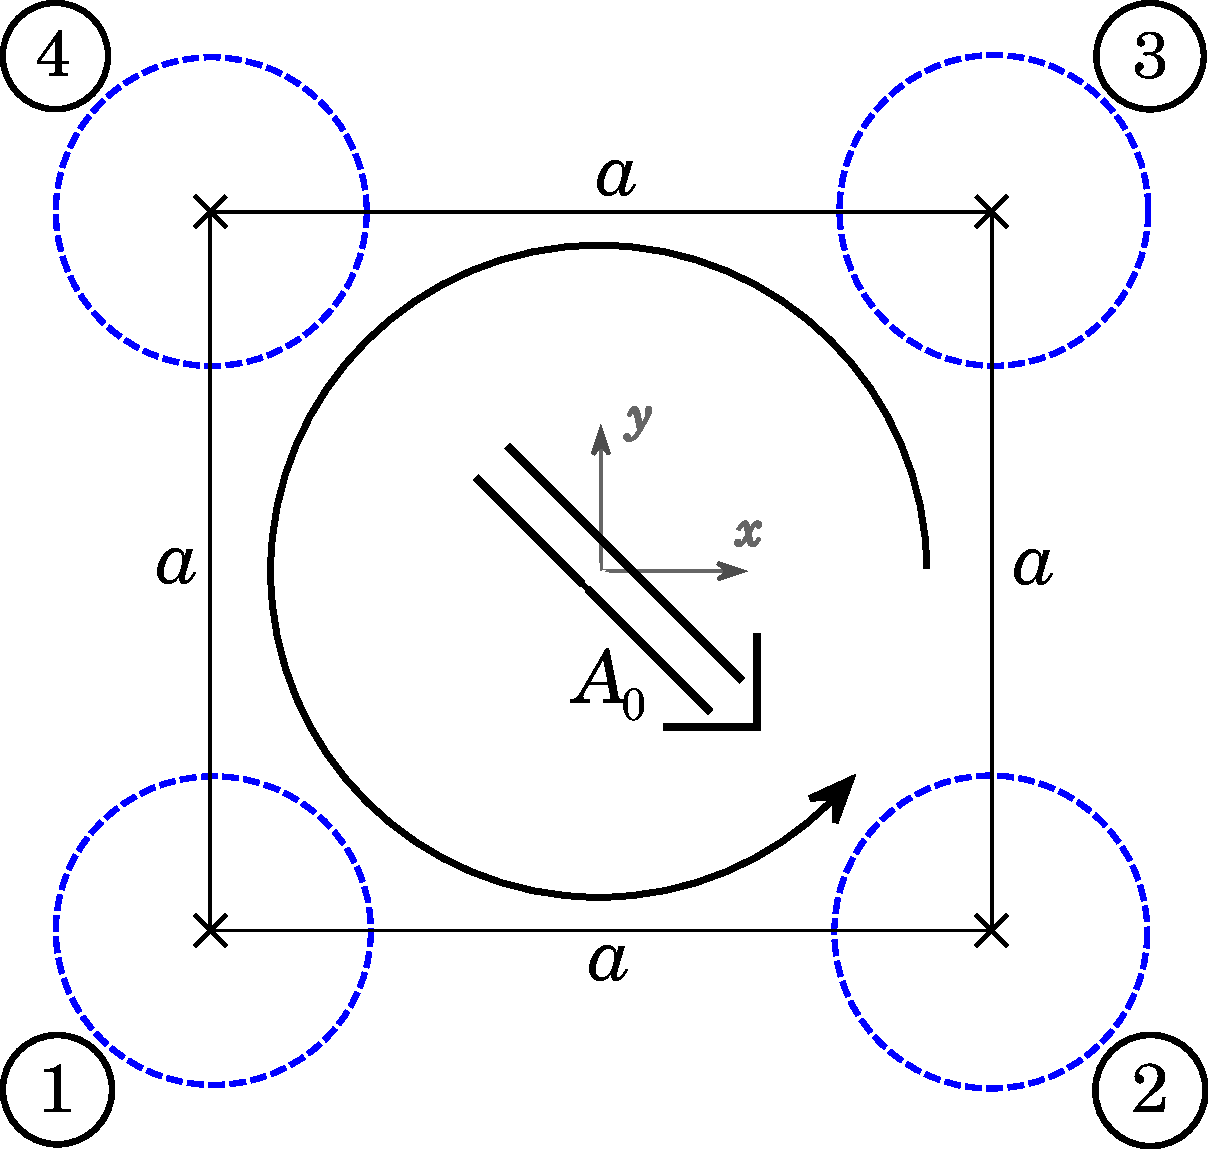
\includegraphics[height = 6cm]{Graphiken/ife_mott_system.pdf}
  \caption{Skizze des rotierenden E-Felds mit der Amplitude $A_0$ zur Modellierung des zirkular polarisierten Lichts im Mott-Hubbard-Isolator. Die Niveaus sind analog zu denen
  in Abbildung \ref{fig:hubbsystem}. Der Koordinaten-Ursprung liegt in der Mitte des Gittersystems und $a$ ist die Gitterkonstante.}
  \label{fig:ifemott}
\end{figure}
Aus dem E-Feld \eqref{eqn:rotefeld} ergibt sich durch Integration der Feldoperator in zweiter Quantisierung
\begin{align}
  H_{\Phi}(t) = q \Phi(t) & = a \sum_{i,\sigma} \left(\vec{r}_i \vec{E}(t) n_{i,\sigma}\right),
  \label{eqn:qPhi}
\end{align}
wobei $q$ die Ladung eines Elektrons, $a$ die Gitterkonstante des Systems und $\vec{r}_i$ der i-te Gitterplatz-Vektor in Einheiten von $a$ ist.
Die Gitterplatz-Vektoren sind in Gleichung \eqref{eqn:gitterplatzvektor} dargestellt. Mit den Gleichungen \eqref{eqn:hamiltonhubb} und \eqref{eqn:qPhi}
ergibt sich der zeitabhängige Hamiltonoperator für den mit zirkular polarisiertem Licht bestrahlten Mott-Isolator
\begin{align}
  H_\text{IFE}(t) = H_\text{Hubb} + a A_0 \sum_{i,\sigma} \left(\left[r_{i,x} \cos{\omega t} + r_{i,y} \sin{\omega t} \right] n_{i,\sigma}\right).
\end{align}
Die $36 \times 36$ - Hamilton-Matrix ergibt sich durch Addition der Hamilton-Matrix für den Mott-Hubbard-Isolator aus Gleichung \eqref{eqn:8N4Ehubbmatrix} mit der Hamilton-Matrix
für das zirkular polarisierte Licht. Letztere beinhaltet nur Diagonalelemente und ist in Gleichung \eqref{eqn:ifematrix} dargestellt.
Im nächsten Schritt wird die Schrödingergleichung \eqref{eqn:schroedingergleichung} wegen der Zeitabhängigkeit des Hamiltonoperators numerisch mit dem Runge-Kutta-5-Integrationsverfahren
gelöst. Dafür werden die folgenden Werte für die auftretenden Parameter eingesetzt:
\begin{align*}
  \text{Tight-Binding-Stärke}&: &J & = \SI{1}{\electronvolt} \\
  \text{Hubbard-Parameter}&: &U/J & \in \{ 4, \, 8 \} \\
  \text{Gitterkonstante}&: &a & = \SI{4e-10}{\meter} \\
  \text{Frequenz\cite{jäckl}}&: &\omega /\tfrac{J}{\hbar} & \in [0.5 , \, 2] \\
  \text{E-Feld-Amplitude\cite{jäckl}\cite{philipp}}&: &A_0 /\tfrac{J}{\symup{e}a} & \in [0.01 , \, 0.1] \\
  \text{Zeitintervall für das E-Feld\cite{jäckl}}&: &t /\tfrac{\hbar}{J} & = [0, \,76]
\end{align*}
Außerdem wird die Anfangsbedingung
\begin{align}
  \ket{\Psi(0)} = \ket{\Psi_0}
  \label{eqn:anfangsbedingung}
\end{align}
gewählt, wobei $\Psi_0$ der Grundzustand des 8N4E-Systems ohne E-Feld ist. Dieser ist für die gewählten Werte von $U/J$
in Tabelle \ref{tab:Upsi0} dargestellt.

Um den zeitabhängigen Stromerwartungswert auszurechnen wird zunächst der Stromoperator aus Gleichung \eqref{eqn:stromoperator} zu
den Basis-Zuständen \ref{tab:8N4Ehubbzust} als $36 \times 36$ - Matrix dargestellt. Diese ist in Gleichung \eqref{eqn:strommatrix} angegeben.
Daraus wird mit dem zeitentwickelten Zustand $\Psi(t)$ der Erwartungswert
\begin{align}
  I(t) = \bra{\Psi(t)} \mathcal{J} \ket{\Psi(t)}
\end{align}
für die Werte
\begin{align}
  A_0 /\tfrac{J}{\symup{e}a} & \in \{0.01,\, 0.05,\, 0.1\} & \omega /\tfrac{J}{\hbar} & \in \{0.5,\, 1.0,\, 1.5, \, 2.0\},
\end{align}
inklusive der Resonanzfrequenzen \eqref{eqn:resofreq}, bestimmt.
Es ergibt sich im gesamten Zeitintervall ein Stromerwartungswert,
der in der Größenordnung $10^{-14} \frac{J\symup{e}}{\hbar}$ liegt und daher als "numerisch Null" interpretiert wird.
Durch das zirkular polarisierte Licht wird also weder zeitabhängig, noch zeitgemittelt ein Strom oder eine Magnetisierung in dem
modellierten Mott-Hubbard-Isolator angeregt.

Um diesen Widerspruch zu der Erwartung einer endlichen Magnetisierung aus Abschnitt \ref{sec:ifeiso} zu erklären, ist in Betracht zu ziehen,
dass das betrachtete Festkörpersystem nicht ausreichend komplex ist, um durch den IFE angeregt zu werden.
Zur Überprüfung dieser Aussage wird im nächsten Schritt der Stromerwartungswert des 8N4E-Systems bei Einschalten des rotierenden E-Felds für $U/J = 0$ untersucht.
In dem Fall, dass das System ausreichend groß ist, um durch den IFE angeregt zu werden, sollte bei $U/J = 0$ ein ein endlicher, stationärer Strom erwartet,
da das System in diesem Fall keinen Mott-Isolator, sondern eher ein leitendes Material modelliert.
Da die Grundzustandsenergie bei $U/J = 0$ vierfach entartet ist, existieren vier unterschiedliche Grundzustände, für die jeweils getrennt
der Stromerwartungswert berechnet wird. Aus dem arithmetischen Mittel der berechneten Erwartungswerte ergibt sich der gesamte
Stromerwartungswert $I(t)$ in Einheiten von $\frac{J\symup{e}}{\hbar}$. Dieser ist in Abbildung \ref{fig:U0plot} gegen die Zeit $t/\tfrac{\hbar}{J}$ aufgetragen.

\begin{figure}
  \centering
  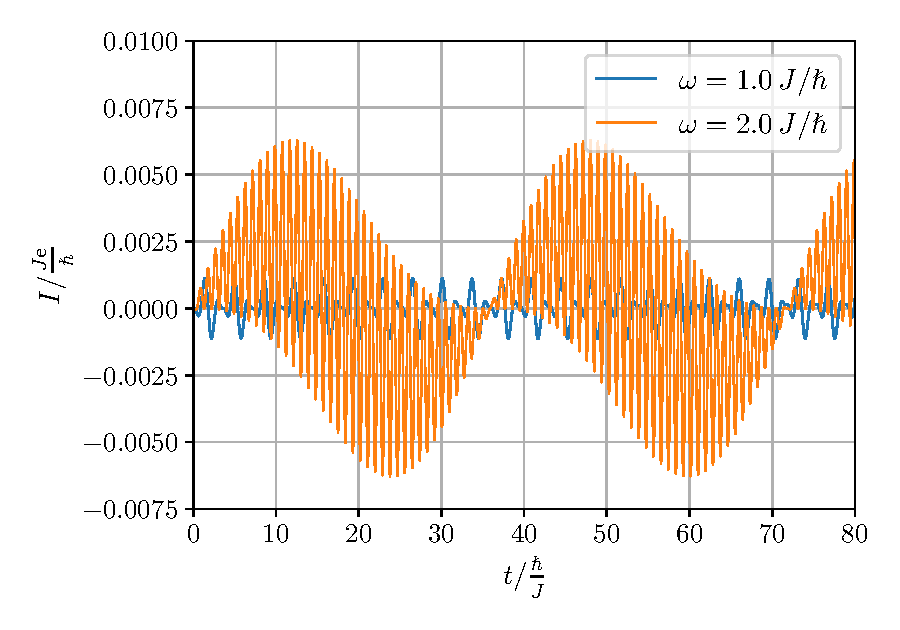
\includegraphics[height=8.0cm]{Plots/U0_E01_schoen.pdf}
  \caption{Stromerwartungswert in Abhängigkeit von der Zeit für zwei verschiedene Frequenzen, wobei $U/J = 0$ und $A_0 = 0.05 \tfrac{J}{\symup{e}a}$ ist.
  Bei $\omega = 2.0\tfrac{J}{\hbar}$ liegt eine Resonanzfrequenz des Systems.}
  \label{fig:U0plot}
\end{figure}

Für die Entstehung der Magnetisierung ist ausschließlich der stationäre, nicht oszillierende Teil des Stroms, der sich aus einer Zeitmittelung ergibt, relevant.
Aus Abbildung \ref{fig:U0plot} ist entnehmbar, dass der Stromerwartungswert periodisch um Null oszilliert und im Langzeitmittel verschwindet. Dies wird für
das Zeitintervall $T/\tfrac{\hbar}{J} \in [0,300]$ numerisch bestätigt.
Es wird daher kein stationärer Kreisstrom durch das zirkular polarisierte Licht mittels des IFE induziert, obwohl das Festkörpersystem bei $U/J = 0$ keinen Mott-Isolator
repräsentiert. Dadurch wird die Behauptung, dass der modellierte Festkörper, bestehend aus vier Gitterplätzen, zu klein für die Untersuchung des IFE ist, gestützt.

Ein weiterer Aspekt, welcher für die Beobachtung eine Rolle spielen könnte, ist die Teilchen-Loch-Symmetrie im System.
Diese wird in der folgenden Betrachtung gebrochen, indem eine Übernächst-Nachbar-Tight-Binding-Wechselwirkung im modellierten Mott-Hubbard-Isolator
ergänzt wird. Dazu werden zusätzliche Tight-Binding-Terme, die das Springen der Elektronen zwischen den Gitterplätzen 1 und 3 bzw. 2 und 4
mit der Stärke $\lambda = 0.2 J$ ermöglichen, ergänzt. Daraus und aus Gleichung \eqref{eqn:hamiltonhubb} ergibt sich der um die Übernächst-Nachbar-Tight-Binding-Wechselwirkung erweiterte Hamiltonoperator
\begin{align}
  H_\text{TL} = H_\text{Hubb} + H_\text{Diag} = H_\text{Hubb} - \lambda \sum_{i=1}^2 \sum_{\sigma} \left(c_{i+2,\sigma}^{\dag}c_{i,\sigma}^{\phantom{\dag}} + c_{i,\sigma}^{\dag}c_{i+2,\sigma}^{\phantom{\dag}} \right).
\end{align}
Mit Hilfe der Basis-Zustände aus Tabelle \ref{tab:8N4Ehubbzust} wird dieser in die Matrix-Darstellung gebracht. Die berechneten $36 \times 36$ - Matrizen für $H_\text{Diag}$ und $H_\text{Hubb}$ sind in den Gleichungen
\eqref{eqn:elmatrix} und \eqref{eqn:8N4Ehubbmatrix} angegeben.
Analog zum ersten Teil dieses Abschnitts wird im System ein hochfrequent rotierendes E-Feld hinzugefügt und der Stromerwartungswert für diverse Parameter berechnet. Im gesamten Zeitintervall ergibt sich
ein Strom, der in der Größenordnung $10^{-15} \frac{J\symup{e}}{\hbar}$ liegt, und daher als "numerisch Null" interpretiert wird. Die im modellierten Mott-Hubbard-Isolator vorhandene
Teilchen-Loch-Symmetrie wird daher nicht für die Beobachtung, dass kein Strom mittels des IFE im System angeregt wird, verantwortlich gemacht.

Die vorangegangenen Untersuchungen deuten darauf hin, dass das betrachtete Festkörpersystem zu klein für die Untersuchung des IFE ist.
Dennoch ist nicht auszuschließen, dass durch die erzielten Ergebnisse die Realität abgebildet wird, sodass in einem Mott-Isolator kein
Kreisstrom durch den IFE angeregt werden kann.
In der in Abschnitt \ref{sec:ifeiso} vorgestellten Herleitung des IFE in Isolatoren werden einige anzweifelbare Annahmen getroffen.
Vor allem die Vernachlässigung von quantenmechanischen Effekten kann in Frage gestellt werden,
da beispielsweise das Vorhandensein des Pauli-Prinzips die Dynamik der Elektronen erheblich beeinflusst kann.
Somit ist nicht eindeutig klar, wie der Widerspruch zwischen der analytischen Herleitung aus Abschnitt \ref{sec:ifeiso} und den Ergebnissen zustande kommt.

\chapter{Zusammenfassung und Ausblick}
\label{ch:ausblick}

Im Rahmen dieser Arbeit werden zunächst die theoretische Grundlagen für das Verständnis der physikalischen und mathematischen Inhalte sowie
verschiedene Isolator-Modelle, insbesondere das Hubbard- und das Heisenberg-Modell, und Herleitungen für den IFE in Metallen und Isolatoren präsentiert.
Durch ein mikroskopisches Festkörpersystem, bestehend aus vier Gitterplätzen und jeweils zwei Spin-Niveaus, wird ein Mott-Hubbard-Isolator modelliert
und untersucht. Der Übergang vom Mott-Hubbard-Isolator in den Mott-Heisenberg-Isolator bei einer besonders starken Coulomb-Wechselwirkung zwischen den Elektronen
$U \gg J$ wird anhand des betrachteten Systems festgestellt und damit die Erwartung bestätigt.
Im nächsten Schritt wird für die Untersuchung des IFE in dem modellierten Isolator ein hochfrequent rotierendes E-Feld eingeschaltet.
Es wird gezeigt, dass kein Strom und somit auch keine Magnetisierung mittels des IFE in dem Festkörpersystem angeregt wird. Der  resultierende Widerspruch
zu der vorgestellten Herleitung für den IFE in Isolatoren lässt vermuten, dass das System für die Nachstellung des IFE in Mott-Isolatoren zu klein ist.
Diese Annahme ist unter anderem darauf gestützt, dass für einen Hubbard-Parameter $U=0$ ebenfalls im Langzeitmittel kein Stromfluss beobachtet wird,
obwohl das Festkörpersystem in diesem Fall keinen Isolator repräsentiert.
Darüberhinaus wird die Vermutung aufgestellt, dass die Teilchen-Loch-Symmetrie des Systems für die Beobachtung, dass kein Strom angeregt wird, verantwortlich ist.
Diese lässt sich jedoch nicht bestätigen, da bei Brechung der Teilchen-Loch-Symmetrie durch das Hinzufügen einer Übernächst-Nachbar-Tight-Binding-Wechselwirkung
weiterhin kein Stromfluss erzeugt wird.
Anhand der aufgestellten Annahmen ist es naheliegend, den IFE in einem vergrößerten Festkörpersystem, wie beispielsweise
in Abbildung \ref{fig:gitterausblick} gezeigt, zu untersuchen. Dabei ist zu beachten, dass mit jedem ergänzten Gitterplatz
die Hilbertraumdimension rapide ansteigt und somit die numerische Auswertung erschwert wird.

\begin{figure}
  \centering
  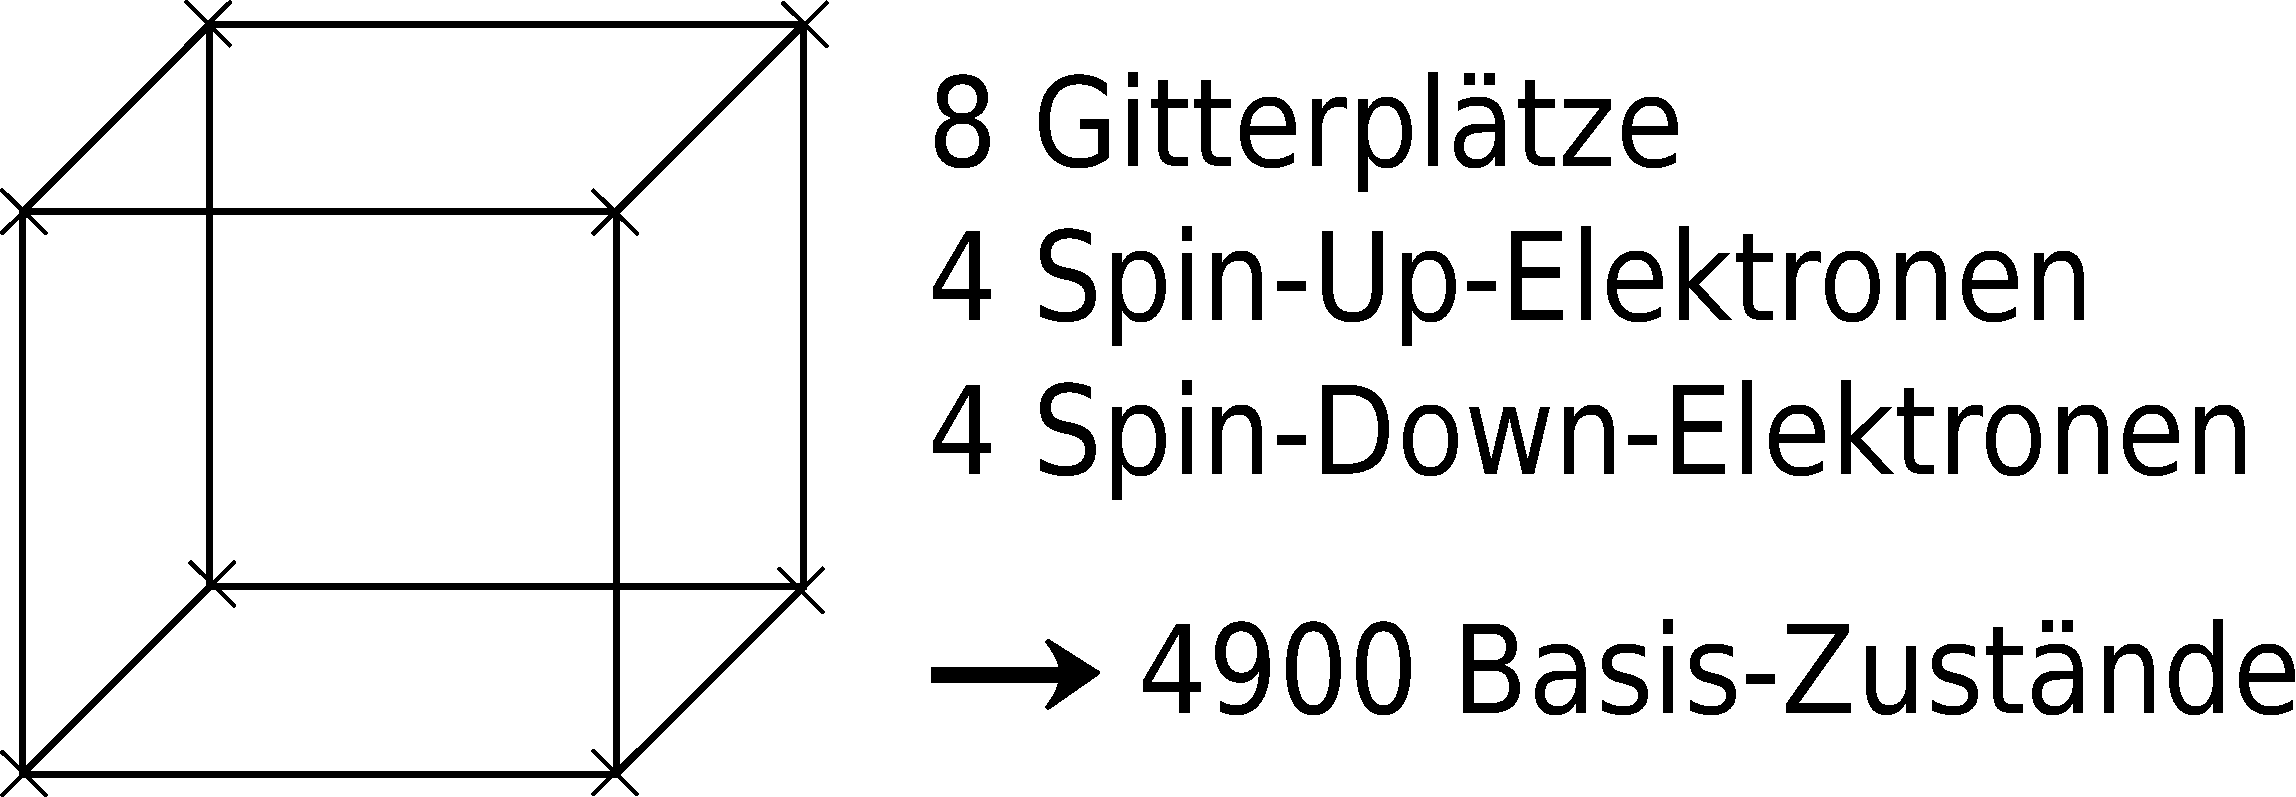
\includegraphics[height=2cm]{Graphiken/gitterausblick.pdf}
  \caption{Eine Möglichkeit zur Erweiterung des Gittersystems.}
  \label{fig:gitterausblick}
\end{figure}

Des Weiteren bleibt die Frage offen, ob durch die in Gleichung \eqref{eqn:isomag} aufgezeigte Formel für den IFE in Isolatoren
die Realität beschrieben wird. Es besteht daher sowohl Interesse an einer Herleitung des IFE, in der quantenmechanische
Effekte berücksichtigt werden, als auch an einer experimentellen Untersuchung des IFE in einem Mott-Isolator.


\appendix
% Hier beginnt der Anhang, nummeriert in lateinischen Buchstaben
\chapter{Ein Anhangskapitel}

Hier könnte ein Anhang stehen, falls Sie z.B. Code, Konstruktionszeichnungen oder Ähnliches mit in die Arbeit bringen wollen. Im Normalfall stehen jedoch alle Ihre Resultate im Hauptteil der Bachelorarbeit und ein Anhang ist überflüssig.


\backmatter
\printbibliography

\chapter{Danksagung}

An dieser Stelle möchte ich mich bei allen bedanken, die mich während der Anfertigung dieser Bachelorarbeit unterstützt haben.

Als erstes gilt mein Dank Herrn Prof. Uhrig für die ausgezeichnete Betreuung meiner Arbeit.
Für die Offenheit für Fragen und die konstruktive Kritik bei der Erstellung dieser Arbeit möchte ich mich ganz herzlich bedanken.
Weiterhin möchte ich mich auch bei Herrn Prof. Stolze für die hervorragende Betreuung und die Beantwortung einer Vielzahl
von Fragen in den letzten beiden Wochen der Anfertigung bedanken.

Ebenfalls möchte ich mich bei meinen Kommilitonen und Mitstreitern Philipp Scherer, Dag-Björn Hering und Matthias Jäger für die gute Zusammenarbeit
bei der Anfertigung unserer Bachelorarbeiten bedanken.

Abschließend bedanke ich mich auch bei meinen Eltern, Geschwistern und Freunden, die mich vor allem in den stressigen letzten Wochen
der Anfertigung großartig unterstützt haben.

Timo Gräßer

\cleardoublepage

\thispagestyle{empty}
\section*{Eidesstattliche Versicherung}
Ich versichere hiermit an Eides statt, dass ich die vorliegende Abschlussarbeit mit dem Titel \enquote{\thetitle} selbstständig und ohne unzulässige fremde Hilfe erbracht habe.
Ich habe keine anderen als die angegebenen Quellen und Hilfsmittel benutzt, sowie wörtliche und sinngemäße Zitate kenntlich gemacht. 
Die Arbeit hat in gleicher oder ähnlicher Form noch keiner Prüfungsbehörde vorgelegen.

\vspace*{1cm}\noindent
\begin{center}
  \begin{tabular}{@{}p{0.4\textwidth}@{\hspace{0.15\textwidth}}p{0.4\textwidth}@{}}
  \rule{\linewidth}{0.25pt}& \rule{\linewidth}{0.25pt}\\
  Ort, Datum & Unterschrift
  \end{tabular}
\end{center}

\subsection*{Belehrung}
Wer vorsätzlich gegen eine die Täuschung über Prüfungsleistungen betreffende Regelung einer Hochschulprüfungsordnung verstößt, handelt ordnungswidrig.
Die Ordnungswidrigkeit kann mit einer Geldbuße von bis zu \SI[round-mode=places, round-precision=2]{50000}{€} geahndet werden. 
Zuständige Verwaltungsbehörde für die Verfolgung und Ahndung von Ordnungswidrigkeiten ist der Kanzler/die Kanzlerin der Technischen Universität Dortmund. 
Im Falle eines mehrfachen oder sonstigen schwerwiegenden Täuschungsversuches kann der Prüfling zudem exmatrikuliert werden \mbox{(\S\,63 Abs. 5 Hochschulgesetz --HG--).}

Die Abgabe einer falschen Versicherung an Eides statt wird mit Freiheitsstrafe bis zu 3 Jahren oder mit Geldstrafe bestraft.

Die Technische Universität Dortmund wird ggf.\ elektronische Vergleichswerkzeuge (wie z.\,B.\ die Software \enquote{turnitin}) zur Überprüfung von Ordnungswidrigkeiten in Prüfungsverfahren nutzen. \\[\baselineskip]

\noindent Die oben stehende Belehrung habe ich zur Kenntnis genommen.\\[1cm]
\begin{center}
\begin{tabular}{@{}p{0.4\textwidth}@{\hspace{0.15\textwidth}}p{0.4\textwidth}@{}}
\rule{\linewidth}{0.25pt}& \rule{\linewidth}{0.25pt}\\
Ort, Datum & Unterschrift
\end{tabular}
\end{center}

\end{document}
